\documentclass[11pt]{report}
\usepackage[utf8]{inputenc}
\usepackage[ngerman]{babel}
\usepackage{amsmath}
\usepackage{bbm}
\usepackage{graphicx}
\usepackage{float}					% erzwingt einen bestimmten grafikplatz
\usepackage[round]{natbib}		% fuer Zitate
\usepackage{hyperref}
\setcounter{secnumdepth}{4}
\setcounter{tocdepth}{4} 



%%\newcommand{\mypapersize}{A4}
\newcommand{\mylaterality}{oneside}

\author{Paul~J.~Arzberger}
\title{Vollautomatische Kalibrierungsmethode hochauflösender Satellitenbildzeitreihen mittels europaweiten MODIS Zeitreihen}

\begin{document}

% Title des articles
\maketitle

\tableofcontents
% ==============================================================================================================
% 
% Motivation
% 
% ==============================================================================================================
\chapter{Motivation}

Zeitreihenanalysen in der Fernerkundung, mit Schwerpunkt zur Change Detection, setzten eine durchgehende, wenn möglich dicht besetzte Ansammlung aus Daten eines oder mehrere Sensoren voraus, um aus dem gesammelten Material einen Informationsgewinn ableiten zu können.


Die Sensoren um das Landsat System stellen einen derartigen Datenfundus zur Verfügung. Die historisch gesammelten Daten von Landsat 5 und 7 sowie von Landsat 8 stellen einen Datenpool von über 30 Jahren Fernerkundungsdaten dar welcher zur Zeitreihenanalyse herangezogen werden kann. 
 Eine weitere Bestrebung kontinuierlich Information über den Zustand der Erde zu liefern stellt das MODIS ( Moderate Resolution Imaging Spectrometer) System mit seinen beiden Satelliten Terra und Aqua dar. In Zukunft werden auch Daten von Sentinel 2 und 3 zur Verfügung stehen welche hochauflösende Daten in periodischen Abständen aufnehmen und im optischen wie im Frequenzband X Daten liefern werden. Anhand der dichten MODIS-Zeitreihe soll nun die Möglichkeit einer vollautomatischen relativen Kalibrierung von Satellitensensoren wie Landsat an die MODIS-Zeitreihe untersucht werden. Die Kalibrierung  stellt eine Prototypenversion, dar welche portabel auf andere Systeme entwickelt werden soll, insbesondere mit Hinblick auf Sentinel 2 und 3. Die entwickelte Software soll rein auf Open Source Produkten /Modulen basieren. In die Kalibrierung fließen nicht nur die Rohdaten sondern auch von LEDAPS generierte Wolkenmasken, welche als Qualitätsparameter und Gewichtung herangezogen werden ein. Die zugrundeliegende MODIS-Zeitreihe wurde zudem noch zusätzlich gefiltert und stellt eine wolkenfreie, mit nahezu keinen NoData-Lücken, europaweite Zeitreihe dar welche zur Kalibrierung herangezogen werden kann. Die Güte der Kalibrierung selbst wird mit einem Qualitätreport beschrieben. 

% ==============================================================================================================
% 
% State Of The Art
% 
% ==============================================================================================================
\chapter{State of the Art}
\section{Filterung verrauschter Satellitenbildzeitreihen}
Satellitenbilddaten können durch atmosphärische Einflüsse wie Dunst, nicht identifizierte Wolkenpixel, Aerosole, gasförmigen Dämpfern etc zusätzlich zu den Effekten des Einfallswinkel und der Illumination verfälscht sein. In den meisten Studien über Phänologie sowie der Bestimmung  von phenologischen Parametern basierend auf Satellitenbilddaten wird als erster Schritt die verrauschte Zeitreihe in eine gefittete Zeitreihe übergeführt.


\subsection{Methoden der Zeitreihenfilterung}
\subsubsection{Savitzky Golay}
Das dem Savitzky Golay Filter zugrunde liegende Polynom ist zweiter Ordnung und die Breite des Moving-Windows der zur Berechnung herangezogenen Daten wird vom User eingegeben. 
\begin{equation}
f(t) = a_0+a_1 \cdot t+a_2 \cdot t^2
\end{equation}

\begin{figure}[H]		% H bedeutet Here
\centering
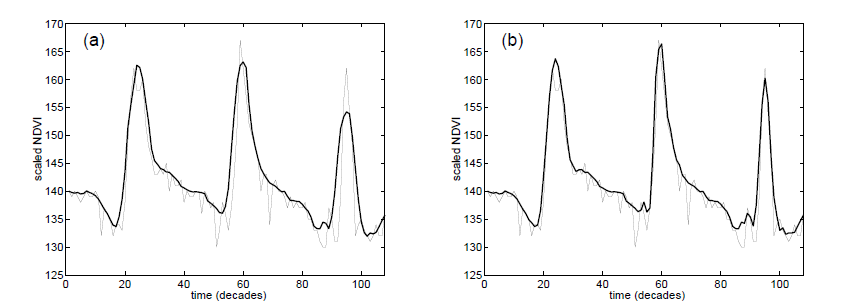
\includegraphics[scale=0.6]{./Grafiken/Fitting/TIMESATmanuell_savitzky_golay_filter.PNG}
\caption{\textit{Gefittete Funktion nach Savitzky Golay. Die dünne Linie repräsentiert die Rohdaten, die dicke Linie repräsentiert die gefittete Funtion. In (a) ist die Moving-Window-Größe n=5, in (b) ist die Moving-Window-Größe n=3 (Eklundh L., Jönnson P.,2012)}}
\end{figure}

\subsubsection{Asymmetrische Gauss'scher Fit}

\begin{equation}
f(t;x_1,\dots,x_5)=\begin{cases} exp \left[-\left(\frac{t-x_1}{x_2}\right)^{x_3}\right] & \mbox{if} \ n  > x_1 
\\ \\
exp\left[-\left(\frac{x_1-t}{x_4}\right)^{x_5}\right] & \mbox{if} \ n  < x_1
\end{cases}
\end{equation}

\begin{flalign}			% flush left align 
t\qquad &\dots\qquad Zeit\\
x_1\qquad &\dots\qquad \text{Position des Maximum oder Minimums} \\
x_2\qquad &\dots\qquad \text{Breite rechte Seite}\\
x_3\qquad &\dots\qquad \text{Wölbung rechte Seite}\\
x_4\qquad &\dots\qquad \text{Breite linke Seite}\\
x_5\qquad &\dots\qquad \text{Wölbung linke Seite}
\end{flalign}

\begin{figure}[H]		% H bedeutet Here
\centering
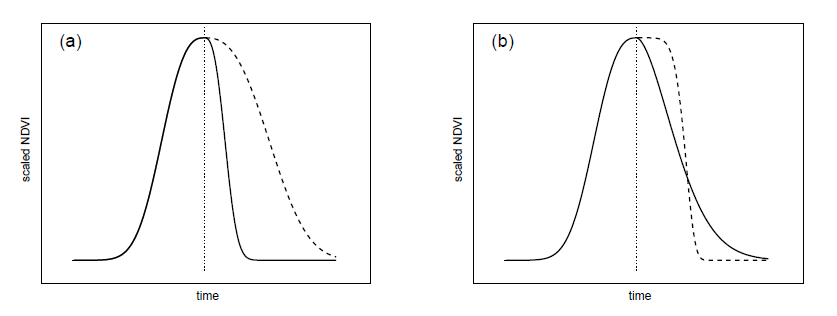
\includegraphics[scale=0.6]{./Grafiken/Fitting/TIMESATmanuell_asymmetric_gaussian_filter.PNG}
\caption{\textit{Auswirkungen auf die Breite und Wölbung wenn sich die lokalen Parameter ändern. In (a) wurde $x_2$ vermindert (durchgezogen) und erhöht ( strichliert),dass sich in einer geänderten Breite und Wölbung auf der rechten Seite auswirkt. In (b) wurde $x_3$ vermindert (durchgezogen) und erhöht (strichliert).(Eklundh L., Jönnson P.,2012)}}
\end{figure}

\subsubsection{Doppel-Logistische Funktion}

\begin{equation}
f(t;x_1,\dots,x_4) = \frac{1}{1+exp\left(\frac{x_1-t}{x_2}\right)} - \frac{1}{1+exp\left(\frac{x_3-t}{x_4}\right)}
\end{equation}


\begin{figure}[H]		% H bedeutet Here
\centering
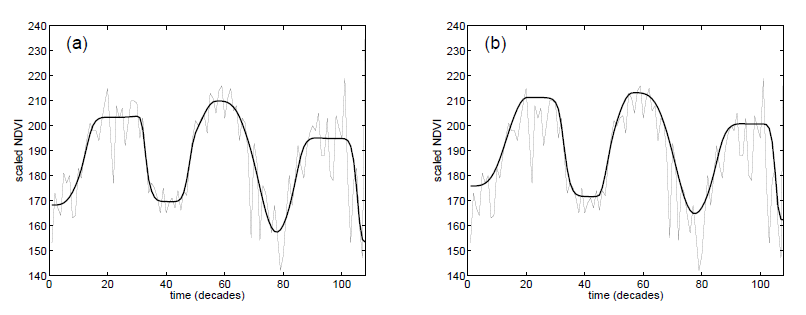
\includegraphics[scale=0.6]{./Grafiken/Fitting/TIMESATmanuell_adaption_to_the_uper_envelope.PNG}
\caption{\textit{Gefittete Funktion nach meheren Iterationen. Die dünne Linie repräsentiert die Rohdaten, die dicke Linie repräsentiert die gefittete Funtion (a). In (b) die erneute Berechnung des Modells mit einer verringerten Gewichtung der niedrigeren Datenwerten (Eklundh L., Jönnson P.,2012)}}
\end{figure}


% Atzberger 2013
\subsubsection{Fourier-Analyse}
Die Diskrete Fourier Transformation ist gegeben durch
\begin{equation}
F_{(u)}=\frac{1}{N}\sum_{t=0}^{N=1}VI(t)\cdot e^{-2\pi ut/T}
\end{equation}
wobei $VI(t)$ in diesem Fall der einzusetzende Wert aus der Zeitreihe zum Zeitpunkt $t$, $n$ die Anzahl der Fourier-Komponenten, $t$ der Periodenindex, $T$ die Gesamtperiodenanzahl wobei diese Zahl gleich der Gesamtanzahl an Epochen in der Zeitreihe. Die obere Gleichung besteht eigentlich aus zwei Zeilen: einem Kosinus-Teil (Realteil) sowie einem Sinus-Teil (Imaginärteil).Die Gleichung für den Kosinus lautet:
\begin{equation}
F_{c(u)}=\frac{1}{N}\sum_{t=0}^{N=1}\left(VI(t)\cdot cos\left(2\pi\frac{ut}{T}\right)\right).
\end{equation}
Die Gleichung für den Sinusteil setzt sich wie folgt zusammen:
\begin{equation}
F_{s(u)}=\frac{1}{N}\sum_{t=0}^{N=1}\left(VI(t)\cdot sin\left(2\pi\frac{ut}{T}\right)\right).
\end{equation}
Aus diesen beiden Gleichungen lassen sich die Phase $F_p$ und die Magnitude $F_m$ berechnen:
\begin{equation}
VI^*(t)=F_{m(0)} + \frac{1}{N}\sum_{t=0}^{N=1}\left(F_{m(n)} \cdot cos\left(\frac{2\pi nt}{T}-F{p(n)}\right)\right)
\end{equation}



% Fitting Methoden aus der Literatur
%
% ==================================================
\subsection{Vergleich unterschiedlicher Fittingmethoden anhand verrauschter Satellitendatenzeitreihen}
Atkinson et al. (2012) wenden anhand des MERIS Terrestrial Chlorophyll Index (MTCI) , ein Vegetationsindex der linear vom Chlorophyllgehalt in überschirmten Flächen abhängt und aus einer MERIS-Zeitreihe abgeleitet wurde, die Diskrete Fourier Transformation, eine Asymmetrische Gauss Funktion, eine Doppel-Logistische Funktion sowie einen Whittaker Smoother auf ihre MTCI-Zeitreihe an. Generell sei vorweg gesagt, dass jede Methode ihre Vor- und Nachteile mit sich bringt, wie sie auf Messfehler oder Ausreisser reagiert beziehungsweise zur Interpretation herangezogen werden kann(de Beurs K.M., Henebry G.M.,2010). \newline
% Grafiken von Arzberger et al einfügen

\begin{figure}[H]		% H bedeutet Here
\centering
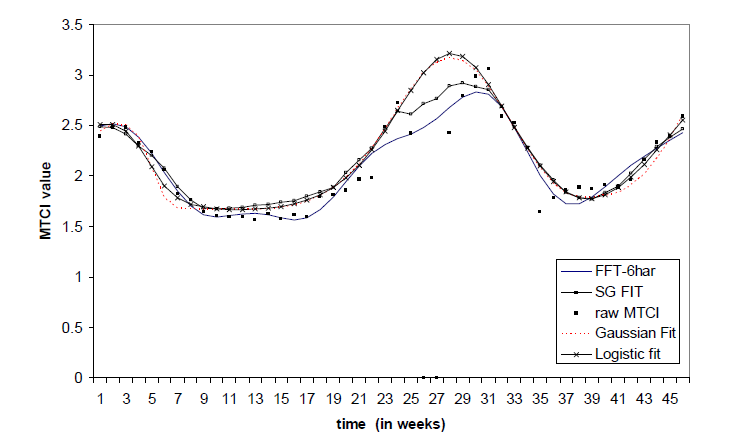
\includegraphics[scale=0.6]{./Grafiken/Fitting/Atkinson_et_al_Vergleich_FFT_SG_LOG_GAU_.png}
\caption{\textit{Vergleich der Fittingmethoden Savitzky-Golay (SG), Gauss'scher Fit, Logistischer Fit (hier mit TIMESAT) und Fourier (FFT) für eine landwirtschaftlich genutzte Fläche in Indien (Atkins et al.,2009)}}
\end{figure}

\begin{figure}[H]
\centering
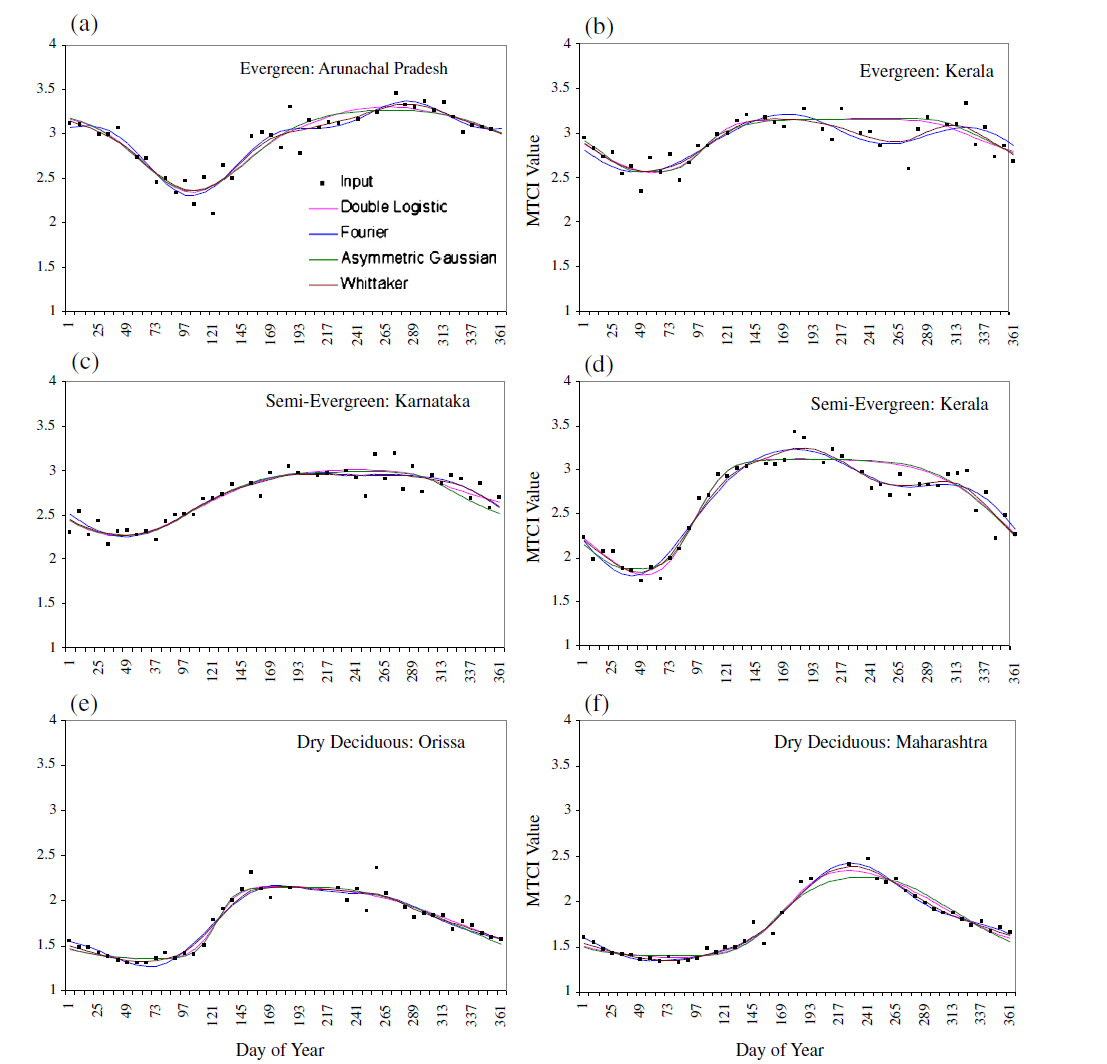
\includegraphics[scale=0.6]{./Grafiken/Fitting/Atkinson_et_al_Vergleich_FFT_SG_LOG_GAU_6locations.PNG}
\caption{\textit{Vergleich der Fittingmethoden Savitzky-Golay (SG), Gauss'scher Fit, Logistischer Fit (hier mit TIMESAT) und Fourier (FFT) anhand von immergrünen Flächen (a,b), semi-immergrünen Flächen (c,d), trockene Laubwälder (e,f)  (Atkins et al.,2012)}}
\end{figure}

\begin{figure}[H]
\centering
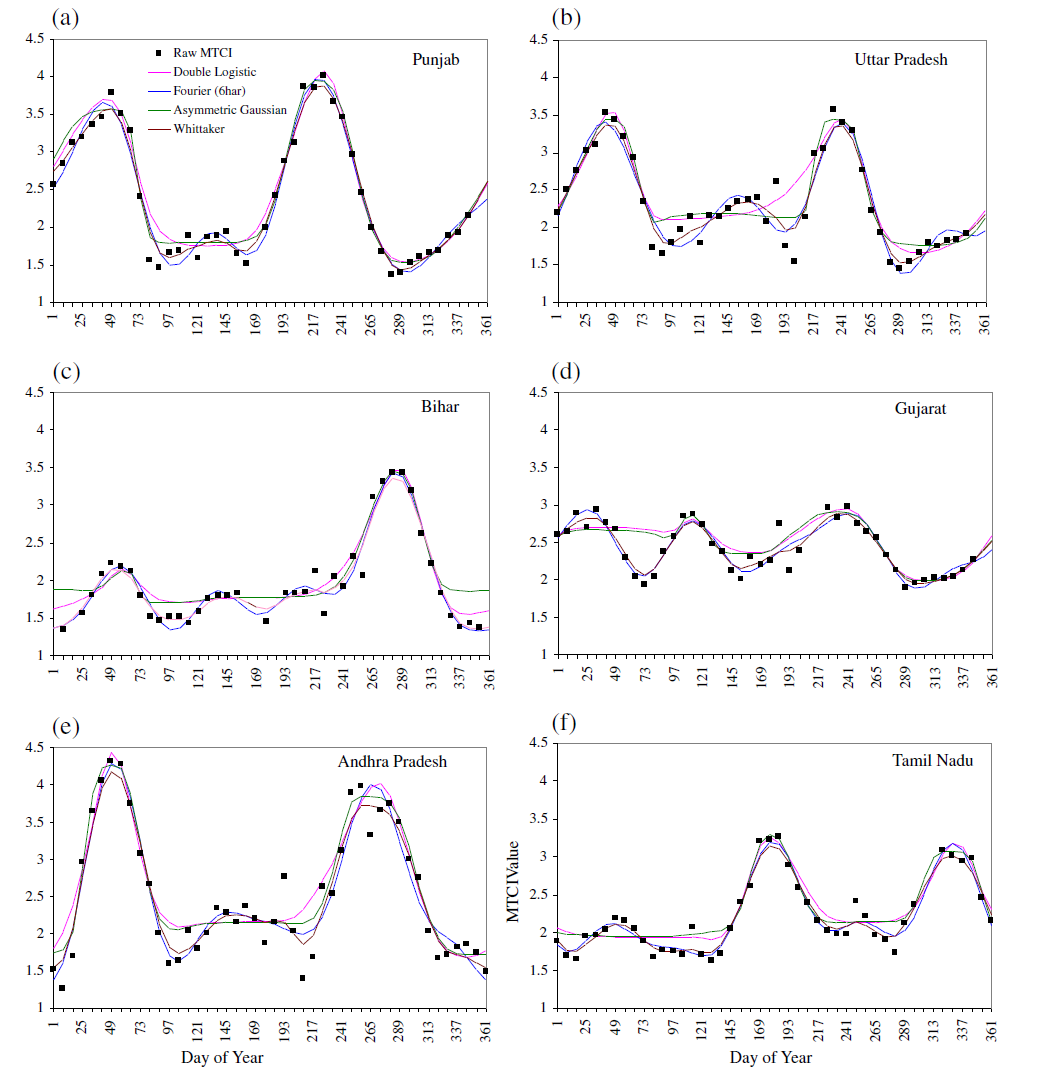
\includegraphics[scale=0.6]{./Grafiken/Fitting/Atkinson_et_al_Vergleich_FFT_SG_LOG_GAU_6locations_agriculture.PNG}
\caption{\textit{Vergleich der Fittingmethoden Savitzky-Golay (SG), Gauss'scher Fit, Logistischer Fit (hier mit TIMESAT) und Fourier (FFT) anhand von landwirtschaftlich genutzten Flächen - Punjab (a), Uttar Pradesh (b), Bihar (c), Gujarat (d), Andhra Pradesh (e), Tamil Nadu (f) (Atkins et al.,2012)}}
\end{figure}





% Pseudo-invariant calibration sites
% ==================================================


% Kalibrierung
% 
% Absolute Kalibrierung
% ==================================================
\section{Kalibrierung}

\subsection{Absolute Kalibrierung}
Unter der absoluten radiometrischen Kalibrierung versteht man die Umrechnung von Digital Numbers (DN) eines Satelliten in physikalische Einheiten in "`am Sensor"' spektrale Strahlung $\left[Wm^{-2}sr^{-1}\mu m^{-1}\right]$. DN eines Senores haben keine Gemeinsamkeiten mit einem anderen Aufnahmesystem. Die Konvertierung zu "`am Sensor"' eintreffende Spektrale Information und Top-Of-Atmosphere Reflexion (TOA) sind fundamentale Vorgehensweisen um die Daten/Produkte zweier unterschiedlicher Sensoren zu vergleichen. 

\subsubsection{Pseudo Invariante Feature Sites - PICS}
Es exitsiert eine Vielzahl an Möglichkeiten von pre-launch laborgetätigten Kalibrationen und post-launch on-orbit Kalibrierungen. Eine der meistverwendeten on-orbit Kalibrierungsmethoden ist die Verwendung von Pseudo Invarianten Calibration Sites (PICS). PICS sind radiometrisch stabile Orte und deren ursprünglicher Zweck der Überwachung der radiometrischen Stabilität eines Sensors mit einem hohen Genauigkeistgrad. Jene Sites zeigen auch hohes Potential unter ähnlicher Genauigkeit zur absoluten Kalibrierung herangezogen zu werden. (5\% Genauigkeit bei Kreuzkalibrierung MSS und Landsat 5 TM laut  Helder et al., 2013). Die zeitliche Stabilität der Libya 4 - Kalibrierungssite wurde anhand des HYPERION EO-1, einem hyperspektralem Erdbeobachtungssensor in hochtransmittiven Spektren des SWIR (bei 1628 nm Wellenlänge ist die Atmosphäre nahezu transparent) untersucht, (siehe Helder et al, 2013)

\begin{enumerate}
\item Sonora Desert - Nord Amerika
\item Lybia 4
\item Sahara
\item Railroad Valley - U.S.A. Nevada
\item Ivanpah Playa - U.S.A. Kalifornien
\end{enumerate}

\begin{figure}[H]
\centering
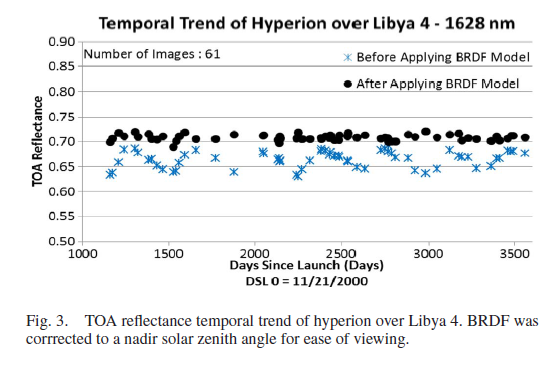
\includegraphics[scale=0.6]{./Grafiken/Abscal/zeitlStabilitaetLybia4_inkl_BRDF.PNG}
\caption{\textit{TOA Reflexion zeitlicher Trend von HYPERION über der Libya 4 Testsite und anhand einer BRDF korrigiert (Helder et al.,2013)}}
\end{figure}

Helder et al wenden zuerst wird ein vereinfachtes lineares BRDF-Modell auf die Libya Testsite an. In diesem Modell wird lediglich der solare Zenithwinkel berücksichtig. Sämtliche anderen Einflüsse werden vernachlässigt.
\begin{equation}
\rho_{Libya4}(\lambda,SZA) = k(\lambda)\rho_h(\lambda)\left[a(\lambda)(SZA)+1\right]
\end{equation}

TOA-Reflexion der Libya4 PICS wird von $\rho(\lambda)$ repräsentiert, $k(\lambda)$ ist der Skalierungsfaktor für das Hyperionspekrtrum, $\rho_h(\lambda)$ ist ein MODIS-Skalierungsfaktor und $a(\lambda)$ repräsentiert den linearen Koeffizienten welcher für die Korrektur des solaren Zenithwinkels benötigt wird.
Die modellierten Werte und die gemessene Beobachtungen unterscheiden sich dabei um 1.3\% (Helder et al., 2013)
Um das Modell zu validieren wurde es auf Landsat 7 ETM+ Daten angewandt. Bei Landsat7 ETM+ wird die radiometrische Genauigkeit/Stabilität auf 5\% angegeben. Da Landsat ein "`am Sensor"' Messlösung ist muss die spektrale Welle die am Sensor gemessen wird, mittels eine Standartprozedur in die TOA übergeführt werden.
\begin{equation}
\rho_\lambda=\frac{\pi\cdot L_\lambda\cdot d^2}{ESUN_\lambda \cdot cos\Theta_s}
\end{equation}
$p_\lambda$ repräsentiert die Oberflächenreflexion $\left[einheitslos\right]$, $L_\lambda$ repräsentiert die spektrale Welle direkt am Sensor $\left[W/(m^2sr\mu m)\right]$, $d$ Erd-Sonnen-Distanz $\left[astronomische Einheit\right]$, $ESUN_\lambda$ repräsentiert die mittlere atmopshärische Solarstrahlung $\left[W/(m^2sr\mu m)\right]$, $\Theta_s$ steht für den solaren Zenithwinkel.
Die Kalibrierungen zeigen bei beiden Sensoren ein Ergebnis das innerhalb ihrer angegeben Ungenauigkeit von 2\% für MODIS und 5\% für Landsat5 ETM+.

\begin{figure}[H]
\centering
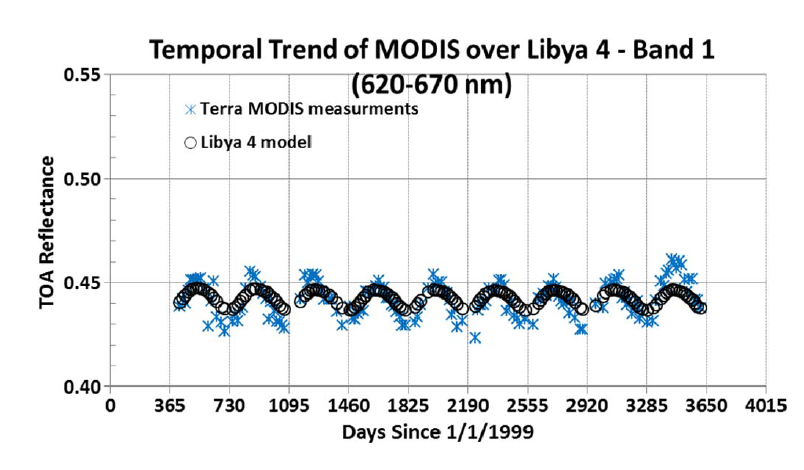
\includegraphics[scale=0.6]{./Grafiken/Abscal/modellierte_gmessene_MODIS_mittels_lin_BRDF_Libya4.PNG}
\caption{\textit{Gemessene MODIS und modelierte MODIS mittels linearer BRDF über Libya4  (Helder et al.,2013)}}
\end{figure}

\begin{figure}[H]
\centering
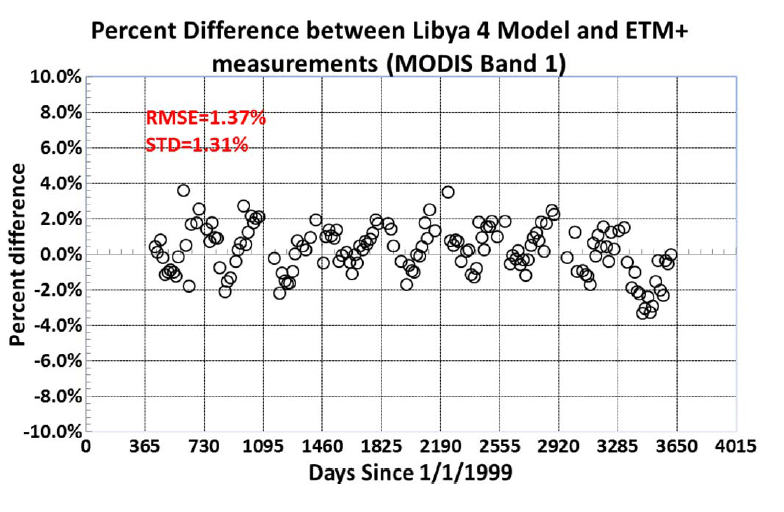
\includegraphics[scale=0.6]{./Grafiken/Abscal/prozent_diff_zw_lyb4model_und_MODIS.PNG}
\caption{\textit{Prozent Differenz zwischen MODIS-Beobachtungen und Modellberechnungen  (Helder et al.,2013)}}
\end{figure}

\begin{figure}[H]
\centering
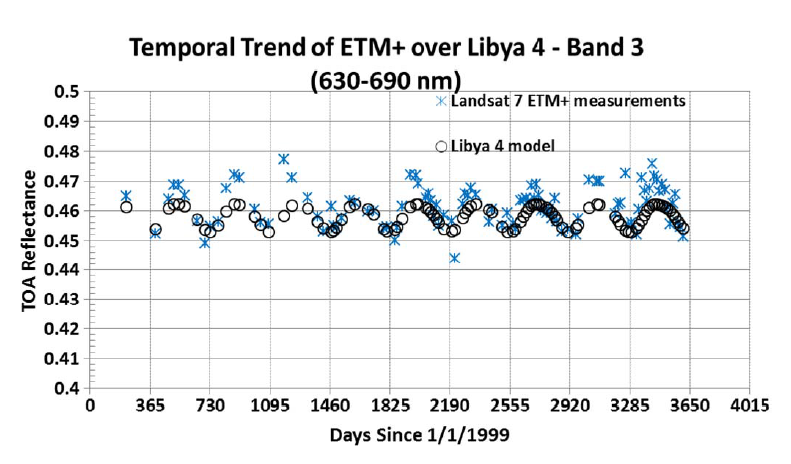
\includegraphics[scale=0.6]{./Grafiken/Abscal/temporaler_Trend_vonETMplus_Libya4.PNG}
\caption{\textit{Gemessene ETM+ (asteriks) und modelierte Prediktionen (kreis) über Libya4  (Helder et al.,2013)}}
\end{figure}

\begin{figure}[H]
\centering
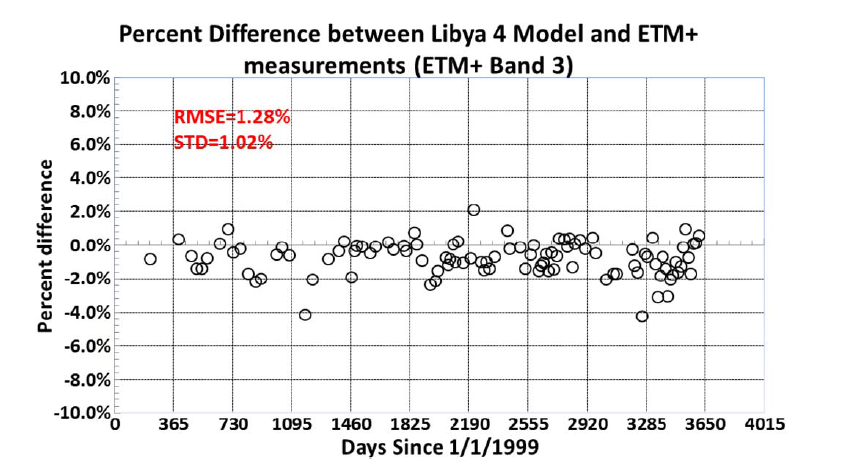
\includegraphics[scale=0.6]{./Grafiken/Abscal/prozent_diff_zw_lyb4model_und_ETMplus.PNG}
\caption{\textit{Prozent Differenz zwischen ETM+ -Beobachtungen und Modellberechnungen  (Helder et al.,2013)}}
\end{figure}

\subsubsection{6S-Modell}
%6S radiative transfer 
% ===============================================
In diesem Unterabschnitt wird grob die 6S Methode zur Berechnung eines empfangenen Signales beschrieben. Für eine genaue Diskussion wird auf die Literatur von Vermote et al., 2006, "`Second Simulation of a Satellite Signal in the Solar Spectrum - Vector (6SV)"' hingtewiesen.\newline\newline
Anhand der 6S (6S - Second Simulation of a Satellite Signal in the Solar Spectrum) radiometrischen Transfer Codes wird der Einfluss der Atmosphäre, speziel die Absorption und Streuung modelliert. Im Idealfall ( mit keiner vorhandenen ) Atmosphäre wird ein Teil der ausgesandten Photonen von der Erdoberfläche absorbiert und der Rest wieder in den Weltraum zurück reflektiert wird. Diese aufgefangenen Messungen selbst hängen direkt mit der Eigenschaft der Reflexionsoberfläche zusammen.bei vorhandener Erdatmosphäre Circa $80 \%$ der Photonen kommen bei einer Wellenlänge von $0.85 \mu m$ und $50 \%$ bei $0.45 \mu m$ an. Jene Lichtteilchen gehen bei zwei Prozessen , der Absorption ( durch Gase, hauptsächlich $ O_2,O_3, H_2O,CO_2,CH_4$ sowie $N_2O$ und der Streuung verloren. Die Absorption ist in der Regel klein gehalten und man vermeidet in der Fernerkundung Bänder in denen stark absorbiert wird. Die Streuung wird durch nicht absorbierende Moleküle verursacht. Das Photon wird dabei in eine andere Richtung reemmitiert in die es eigentlich weiter gehen sollte. In der Regel durchläuft ein Photon mehrere solche Streuungsvorgänge, welche in der Verarbeitung mitberücksichtigt werden müssen.\newline
Ein Teil der Strahlung wird direkt von der Atmosphäre zurück reflektiert ohne die Oberfläche zu erreichen somit tragen sie nur zum Strahlungshaushalt bei aber nicht zum Informationsgewinn über das Beobachtungsziel. Die überbleibenden Photonen beleuchten die Oberfläche abhängig von ihrem gestreuten Pfad diffus und werden auf ihrem Weg Richtung Weltraum bzw Sensor erneut gestreut, reflektiert und erneut gestreut ( Trappingeffekt ). Kurz es verlangt nach einer genauen Bestimmung der absorbierenden Gase der Atmosphäre sowie eine genaue Behandlung der Streuprozesse in Kombination beider Prozesse. \newline

\addcontentsline{toc}{subsubsection}{Absorptions- und Streuungseffekte} 
\subsubsection*{Absorptions- und Streuungseffekte}
%Elektronische Veränderungen , oder besser Elektrostatische Veränderungen???
Die absorbierenden Gase Sauerstoff ($O_2$), Kohlendioxid ($CO_2$), Methan ($CH_4$) und Distickstoffmonoxid ($N_2O$) werden als Konstant in der Atmosphäre angenommen. Wasser ($H_2O$) und Ozon ($O_3$) werden als zeit- und ortsabhängig betrachtet. Gase Absorbieren Strahlung indem sie ihre Rotations, Vibrations- sowie Elektronischen Zustände verändern.
Veränderungen der Rotation werden im Mikrowellen oder fernen Infrarot sichtbar und sind typisch für schwache Frequenzen. Veränderungen in der Vibration sind im Nahen Infrarotbereich angesiedelt. Elektronische Veränderungen können im sichtbaren und ultravioletten Bändern sichtbar gemacht werden. Die Absorptionskoeffizienten variieren sehr stark mit der unterschiedlichen Wellenlänge und stellen ein sehr komplexes Konstrukt dar. $H_2O$ beeinflusst hauptsächlich Wellenlängen die größer als $0.7 \mu m$sind.  $O_3$ hat seine größte Absorptionsfähigkeit zwischen $0.55 - 0.65 \mu m$ und limitiert die Erdbeobachtung auf Wellenlängen größer $0.35 \mu m$. $CO_2$ beeinflusst Wellenlängen größer $1\mu m$ jedoch nicht so stark wie $H_2O$ und wirkt störend auf den Wasserdampf. $O_2$ stärkster Einfluss ist um ca $0.7 \mu m$, $CH_4$ zeigt besonders starken Einfluss bei $2.3$ bzw bei $3.35$, $N_2O$ hat ebenfalls in zwei Bereichen einen starken Einfluss und zwar bei $2.9 \mu m$ und $3.9\mu m$.\newline\newline

Bei der Annahme das die Oberfläche einheitliche lambertsche Reflexionseigenschaften aufweist und die Atmospäre horizontal einheitlich geschichtet ist wird die Reflexion als 
\begin{equation}
\rho^*=\frac{pi L}{\mu_s E_s}
\end{equation} \newline

\begin{flalign}			% flush left align 
L\qquad &\dots\qquad \text{gemessene Strahlung}\\
E_s\qquad &\dots\qquad \text{solare Flux am Atmosphären-beginn} \\
%\mu_s = cos(\Theta_s)\qquad &\dots\qquad \text{\Theta_s  Sonnenzenitwinkel}\\
\end{flalign}\newline

% aus den 6S manual vom vermote part 1
Berücksichtigt man atmopshärischen Einfluss, Absorbtionseffekte von $H_2O, O_2, CO_2$ und $O_3$, Streuung an Molekülen und Aerosolen und der Einfluss der Oberfläche, schreibt man nun \newline (Vermote et al, 6S,2006)s
\begin{equation}
\rho' (\Theta_s, \Theta_v, \Phi_v) = t_g ( \Theta_s, \Theta_v) \left\{\rho_a(\Theta_s, \Theta_v, \Phi_v)+ \frac{T(\Theta_s)}{1-\langle\rho (M)\rangle S}\left[  \rho_c(M)e^{-\tau / \mu_v} + \langle \rho(M)\rangle t_d(\Theta_v)\right] \right\}
\end{equation}\newline
Auf eine genaue Diskusion wird 
Um eine erfolgreiche Kalibrierung mittels der 6S Methode durchführen zu können benötigt man Infromationen über 
\begin{itemize}
	\item geometrische Zustände der Strahlungsquelle und Sensor
	\item atmosphärische Modellierung der Gaskomponenten
	\item das Aerosolmodell
	\item spektralen Zustände
	\item die Bodenbeschaffenheit (Typ und Variation)
\end{itemize}
Für jeden Schritt in der Berechnung werden entweder standartisierte Zustände angenohmen oder selbsdefinierte fliessen ein. Die Satellitenposition wird generell als grob angenommen.

\begin{figure}[H]
\centering
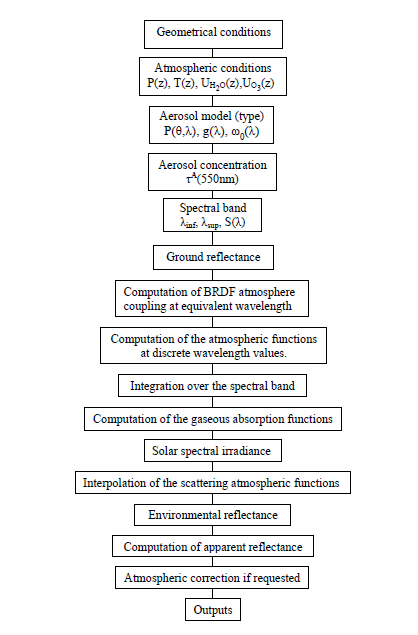
\includegraphics[scale=0.6]{./Grafiken/Abscal/Workflow_6S.PNG}
\caption{\textit{Workflow der 6S Radiative Transformation Codes  (Vermote et al.,2006)}}
\end{figure}

%BRDF - aus Einige BRDF Modelle
% ===============================================
\subsubsection{Bidirektionale Reflektionsverteilunsgfunktion}

Die Bidirektionale Reflektionsverteilungsfunktionen (BRDF) beschreiben die Reflektionseigenschaften von Materialien und Oberflächen und Berücksichtigt den Einstrahlwinkel des Emitters sowie den Blickwinkel des aufnehmenden Sensors. Verschieden Materialien reflektieren bei gleicher Beleuchtung unterschiedlich. Manche Oberflächen zerstreuen das einfallende Licht difus während andere wiederum die Strahlung als Spiegel reflektieren. Generell geben sie an wie viel Licht von einer Oberfläche reflektiert wird abhängig von der pyhsikalischen Beschaffenheit (Wellenlänge) des ausgesendeten Lichtes sowie der Oberflächenbeschaffenheit und Zusammensetzung der reflektierenden Materie.\newline

Die BRDF ist eine Funktion in vier Variablen
\begin{equation}
BRDF = f(\Theta_{in},\Phi_{in},\Theta_{ref},\Phi_{ref}) = f(\mathbf{L},\mathbf{V})
\end{equation}\newline

wobei $\Theta_{in}$, $\Phi_{in}$, $ \Theta_{ref}$, und $\Phi_{ref}$ die Azimuth- und Deklinationswinkel der Einfalls- und Reflexionswinkel bezüglich der Strahlunsquelle sowie des Sensors sind.  \textbf{\emph{L}} bezeichnet dabei die Richtung der Lichtquelle und \textbf{\emph{V}} die Richtung des Senors auf die Oberfläche. Ohne jetzt weitere Einflussparameter zu nennen oder in die Tiefe zu gehen  siehe [N. Gebhardt] beschreibt einen BRDF für eine speziel definierte Wellenlänge das Verhältnis zwischen der differentiellen Leuchtdichte \textbf{\emph{$ Radiance dL_{ref}$}} in Beobachtungsrichtung und der differentiellen Bestrahlungsstärke \textbf{\emph{$ Irradiance dE_{in}$}} die aus der Beleuchtungsrichtung auf die beschienene Oberfläche wirkt, beschreibt.

\begin{equation}
BRDF(\Theta_{in},\Phi_{in},\Theta_{ref},\Phi_{ref}) = \frac{dL_{ref}(\Theta_{ref},\Phi_{ref}}{dE_{in}(\Theta_{in},\Phi_{in})}
\end{equation}
\newline
%Grafiken einfügen von "Basic Principles of Surface Reflectance"


Allgemein ist die BRDF eine Funktion die nur in drei Variablen abhängig ist $f(\Theta_{in},\Theta_{ref},\Phi_{in}-\Phi_{ref}) $. Als weiterführende Literatur wird Nikolaus Gebhardt und Shree Nayar empfohlen.
\newline
Die Oberflächenalbedo variiert sehr stark abhängig von sesonalen oder geographischen Parametern. Regenfall kann zum Beispiel die Oberflächenalbedo einer Baumkrone um bis zu 50\% reduzieren (Román et al 2009). Zusätzlich dazu kommen noch Faktoren wie Schattenwurf durch Baumkronen oder spiegelnde Reflexionen abhängig vom Einfallwinkel des Sonnenlichtes oder atmosphärische Veränderungen und Schwankungen (Román et. al. 2009).\newline

%BRDF - MODIS collection V005 BRDF/albedor product
\subsubsection{MODIS ( Collection V5) BRDF/albedo product}
%Román et Al, 2009
Der Algorithmuis beruht auf multitemporalen, wolkenfreien, atmosphärisch korregierten Oberflächenreflexionen der Terra und Aqua Satelliten um die Anisotropie der Oberflächenreflexion über eine 16 Tage lange Periode zu modellieren.
Verwendet wird dabei ein kernelbasiertes lineare Modell der BRDF auch bekannt als Ross-Lick/Li-Sparse-Reciprocal kernelartiges BRDF-Modell. Dieses Modell beruht auf den gewichteten Summen eines isotropischen Parameters sowie zwei Funktionen (oder Kernel) abhängig von Blickrichtung und Illumination. $\Theta$ steht für den solaren Zenithwinkel, $\vartheta$ Winkel unter dem der Pixel betrachtet wird, $\Phi$ ist der relative sonnengerichtet Azimuth in Blickrichtung des Senors und $\Lambda$ ist das solarspektrale gewichtete Zentrum für ein gegebenes MODIS Band

$f_{iso}(\Lambda)$ ist die isotropische Streuungskomponente und gleich der bidirektionalen Reflexion bei einem Betrachtungswinkel von $\vartheta=0$ und dem solaren Zenithwinkel $\Theta=0$. $f_{geo}(\Lambda)$ ist der Koeffizient für des Li-Sparse-Reziproken geometrischen Streungskerne $K_{geo}$ welcher sich aus der Oberflächenstreuung und der geometrischen Schattenwurf Theorie herleitet. Der Parameter $f_{vol}(\Lambda)$ ist der Koeffizient des Ross-Thick Volumens-Streuungskernel $K_{vol}$, welcher sich aus radiativen Transfermodellen. Die best gefitteten Ross-Thick/Li-Sparse-Reziproken (RTLSR) Modellparmater werden an den ersten sieben MODIS Spektralbändern angebracht. Zusammengesetzt sieht das Modell wie folgt aus
\begin{equation}
R(\Theta,\vartheta,\Phi,\Lambda) = f_{iso}(\Lambda) + f_{vol}(\Lambda)K_{vol}(\Theta,\vartheta,\Phi) + f_{geo}(\Lambda)K_{geo}(\Theta,\vartheta,\Phi).
\end{equation}
Anhand von Integration über alle Blickwinkel ergibt sich ein Modell für einen direkte hemisphärische Reflexion (DHR) oder Black-Sky-Albedo (BSA). Die Integration über alle Illuminationswinkel führt zur Bihemisphärischen Reflexion ( BHR) unter isotropischer Illumination oder einer White-Sky-Albedo (WSA).\newline

\begin{equation}
BSA(\Theta_s)=\sum_{N}^{}f_kh_k(\Theta_s)
\end{equation}

\begin{equation}
WSA = \sum_{k}f_kH_k
\end{equation}

$h_k(\Theta)$  stellt das Integral des BRDF Kernels $k$ über einen gegebenen Beobachtungszenith und (...weiterschreiben / vergleich der Intergrationsparameter mit den Allgemeinen BRDF Parametern)




\subsection{Relative Kalibrierung}
\subsubsection{Lineare Regression}
(Tokol T. et al, 1999) gehen von zwei Grundlegenden Strategien aus, die bei der relativen Datenkalibrierung angewandt werden können. Manche Methoden basieren auf der Verteilung der Bildinformation während andere auf paarweise Pixelbeziehungen abziehlen. Alle Regressionsmodelle wurden anhand von robusten Methoden berechnet, welche iterativ die Gewichte für die Regression neu berechnen. Um Band-zu-Band kalibrieren zu können wird folgendes Modell verwendet:
\begin{equation}
\hat{y_i}=\beta_0+\beta_1x_i
\end{equation}
$y_i$ ist hierbei ein Pixel eines Bandes aus einer nachfolgenden Epoche und $x_i$ bezieht sich auf einen Pixel eines Bandes in einer früheren Epoche. (Vermote E.F., Saleous N.Z., 2006) führen einen Kreuzkalibrierung zwischen AVHRR und MODIS über einem radiometrischen stabilem Wüstengebiet im Niger anhand einer lineraren Translation durch.


\subsubsection{PIF's}

In dieser Diplomarbeit werden als Ausgangsdaten der radiometrischen Kalibrierungsmethode mittels LEDAPS absolut kalibrierte Landsatdaten verwendet. 
Die Cross-calibration zweier Sensoren über einem radiometrisch stabilen Gebiet wird in der Literatur häufig angeführt. Bei diesen Pseudo-Invariant-Calibration Sites handelt es sich wiederholt um die selben Gebiete. Diese Sites wurden eigentlich dafür ausgesucht um die Langzeitstabilität eines Sensors zu überprüfen. Um die DN der Landsatdaten 


% SOFTWARE
% 
% LEDAPS
% ==================================================
\section{Bestehende Software}
\subsection{LEDAPS - Landsat Ecosystem Disturbance Adaptive Processing System }
Das Landsat Ecosystem Disturbance Adapticve Processing System (LEDAPS) wurde ursprünglich im Jahre 2006 von der National Aeronautics and Space Administration - Goddard Space Flight Center und der Universität von Maryland entwickelt um Top-Of-Atmosphere (TOA) Reflexionsprodukte aus Daten der  Landsat Thematic Mapper (Landsat5) und dem Enhanced Thematic Mapper Plus Level1 (Landsat7) Sensoren zu generieren. Der in dieser Diplomarbeit verwendete Algorithmus wurde vom USGS für den Landsat Surface Climate Data Record angepasst.
LEDAPS setzt sich aus sechs Modulen zusammen die drei Schlüsseloperationen beinhalten.

% TOA ist einheitslos ( apparent reflexion) (Pahlevan Nima, 2012) auf Seite 171 absatz conversion to Toa reflectance
\begin{enumerate}
\item Konvertierung von Digital Numbers (DN) zu TOA Reflexionen
\item Wolkenpixeldetektion anhand der TOA
\item Transformation der TOA zu Oberflächenreflexion mittels zusätzlichen Daten
\end{enumerate}

Die atmosphärische Korrektur wird anhand eines 6S-Korrekturmodells gerechnet welche Druck, Wasserdampf, Ozon sowie geometrischer Höheninformation. 
\begin{figure}[H]
\centering
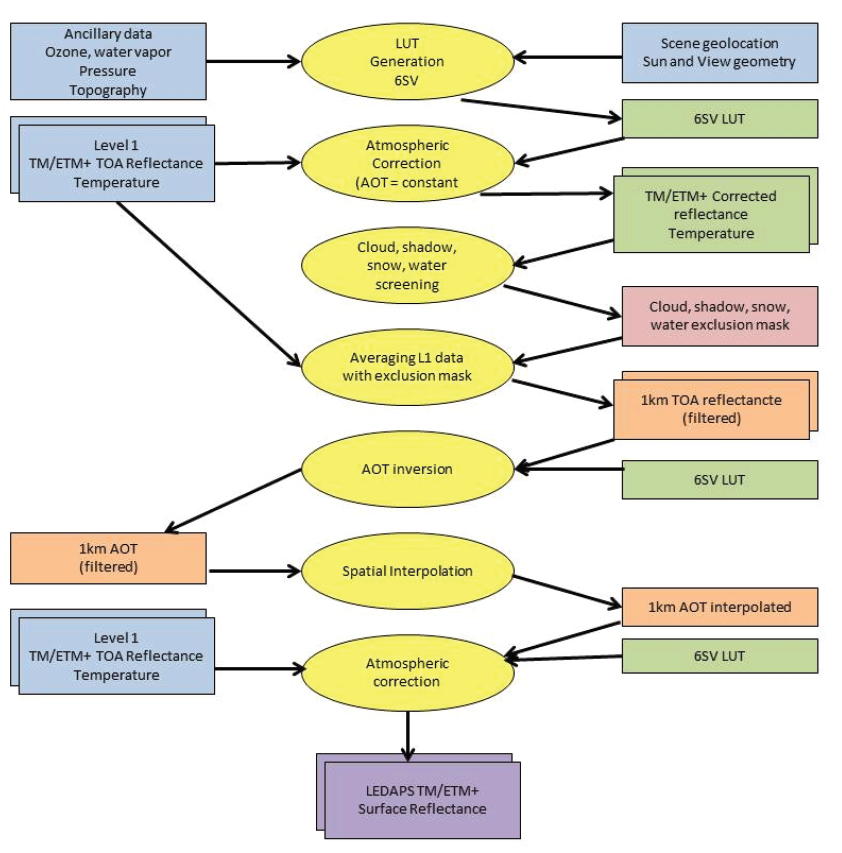
\includegraphics[scale=0.6]{./Grafiken/LEDAPS/Atmospheric_correction_flow_LEDAPS.PNG}
\caption{\textit{Workflow der atmosphärischen Korrektur, (U.S.G.S., 2013)}}
\end{figure}
%Dies wird dazu verwendet um die Größe der atmosphärischen Dicke zu berechnen. 

Für diese Diplomarbeit von besonderer Bedeutung ist die Qualitätsinformation die im gesamten Vorgang erstellt wird und weiterführend als Wolkenmaske verwendet wird. Das Modul 5 umfasst sämtliche Bearbeitungsschritte die zur Wolkendetektion verwendet werden. Hierfür werden die Bänder 1,3,4, und 6 sowie Zusatzinformation wie Lufttemperatur, Solarzenith, Solarazimuth etc zur Bestimmung verwendet. Sämtliche akquirierte Daten der Systeme Landsat5 TM und Landsat7 ETM+ werden in einem Vorverarbeitungsschritt diesem Algorithmus unterzogen. 
\begin{figure}[H]
\centering
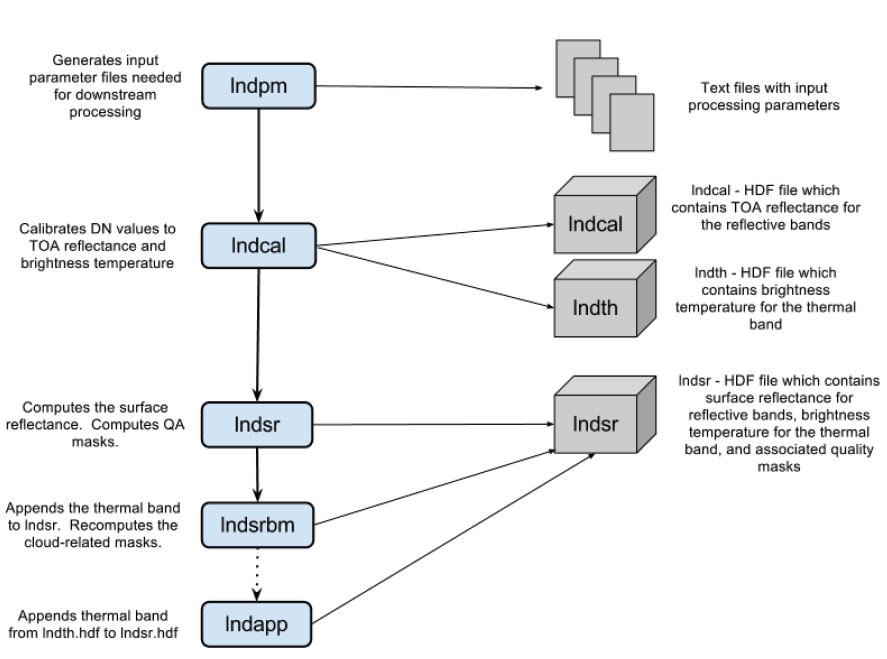
\includegraphics[scale=0.6]{./Grafiken/LEDAPS/Algorithm_workflow_LEDAPS.PNG}
\caption{\textit{Workflow des LEDAPS-Algorithmus, (U.S.G.S., 2013)}}
\end{figure}


Als Endergebnis liegen Landsat5 TM und Landsat7 ETM+ Daten als Oberflächenreflexion im hdf-Format vor. 

%TIMESAT
% ==================================================

\subsection{TIMESAT}
TIMESAT wurde primär zur Prozessierung von Vegetationsindexzeitreihen für die  Ableitung von saisonalen Parametern wie Anfang, Ende, Länge etc der Vegetationsperiode entwickelt. Es erlaubt die Filterung von Satellitenbildzeitreihen sowie berücksichtigt es Zusatzinformation wie Qualitätsinformationen ( z.B. Modis Qualitätsprodukt) für eine mögliche Gewichtung. Die verwendeten Algorithmen basierend auf der Methode der kleinsten Quadrate sind ein Savitzky Golay Filtern sowie zwei Methoden bei denen die Daten anhand von nonlinearer Funktionen unterschiedlicher Komplexität gefittet werden. TIMESAT arbeitet iterativ und mit einer dynamischen Gewichtung. Nach einer ersten Iteration und Schätzung der Parameter werden die Rohdatenwerte unterhalb der gefitteten Kurve mit einem neuen geringeren Gewicht behaftet und das Modell wird neu berechent. Dadurch resultiert eine an den oberen Verlauf der Daten adaptiertes Modell.TIMESATs größter Nachteil ist die Prozessierungsgeschwindigkeit. In der Literatur wird TIMESAT meist nur für kurze Perioden oder einem beschränkten Gebiet eingesetzt siehe (Jönsson P., Eklundh L.,2004) sowie (Tan B. et al.,2011). Bei der Prozessierung einer Zeitreihe die Daten von mehr als einem Jahrzehnt umfasst steigt die Rechenzeit und das Programm wird nicht mehr brauchbar. 


% ==============================================================================================================
% METHODIK
% Grundlagen
% 
% ==============================================================================================================




\chapter{Methodik}
% MODIS - Allgemeine Informationen
% - to do: was über die einheiten schreiben , warum modis, weil SI einheiten verwendet wie bei Landsat etc ( schauen in Tokola 2013 
% ================================

\section{Datengrundlagen}
In diesem Kapitel werden die verwendeten Satellitendaten besprochen. Dabei handelt es sich um multispektrale Satellitendaten unterschiedlicher Auflösung und Datengehaltes  sowie der Qualitätsinformation die bei der absoluten Kalibrierung der Landsatdaten mittels LEDAPS generiert wurde als fertiges Produkt für MODIS bereitgestellt wird. 



% MODIS - stabilität in den sichtbaren bändern
% ==========================================================================
% Da laut Vermote und Saleous die Pixelgröße der beiden zu Kalibrierenden Daten (AVHRR/MODIS) ab einem zenitwinkel von größer50 Grad zu unterschiedlich werden, klammern sie dies aus. Randpixel ausmaskieren kann eventuell eine steigerung der Genauigkeit bedeuten. Helder et al 2013 verweist auf seite 1363 das grosse zenithwinkel ( die nicht spezifiziert wurden ) und winkel größer 15° in der backscatter direction ausgelassen werden sind Kalibrierungsergebnisse kleiner 1% möglich


% Landsat
% ==========================================================================
\subsection{Landsat - Allgemeine Informationen zum Sensor und Trägersystem}
Landsat ist die weltweit längste zivile Erdbeobachtungsmission mittels Fernerkundungssensoren  mittlerer Auflösung. Seit 1972 sind bis jetzt 8 Satelliten in Orbit gebracht worden wobei Landsat 6 beim Start verlorenging. Im näheren wird nur auf jene Sensoren eingegangen deren Daten in der Diplomarbeit verwendet wurden. Dies umfasst die Satelliten Landsat5, Landsat7 und Landsat8.

Landsat5 und Landsat4 (der Vollständigkeit halber erwähnt) wurden mit den verbesserten \textit{Thematic Mapper} ausgestattet der im sichtbaren Bereich und nahen Infrarotbereich sowie im thermalen und panchromatischen Bereich Aufnahmen tätigt. Für das sichtbare und naheinfrarote Spektrum beträgt die Auflösung 30m, für das thermale Band 120m und im panchromatischen Kanal 15m.

Landsat7 führt den multispektralen \textit{Enhanced Thematic Mapper Plus} (ETM+) mit sich, welcher im sichtbaren Bereich und nahen Infrarotbereich sowie im thermalen und panchromatischen Bereich Aufnahmen tätigt. Für das sichtbare und naheinfrarote Spektrum beträgt die Auflösung 30m, für das thermale Band 60m und im panchromatischen Kanal 15m.
Der Satellit führt drei on-board Kalibriereinrichtungen mit sich einen \textit{Full Apertrure Solar Calibrator(FASC)}, einen \textit{Partial Aperture Solar Calibrator (PASC)} und einen \textit{Internal Calibrator (IC)}

Landsat8 wurde mit dem multispektralen Sensor \textit{Operational Land Imager} (OLI) und dem \textit{Thermal Infrared Sensor} (TIRS) ausgestattet. OLI liefert Aufnahmen in 8 spektralen Bändern in einer Auflösung von 30 m und einem panchromatischen Kanal in einer Auflösung von 15m. TIRS nimmt in zwei mittleren infraroten Bereichen in einer Auflösung von 100m auf. Da die TIRS Daten allerdings mit den OLI-Daten mitgeliefert werden, werden sie auf 30m neu aufgelöst.

Aktuell liefern Landsat7  und Landsat8  alle 16 Tage Aufnahmen des selben Erdoberflächenausschnittes. Die Orbits sind polare, sonnen-synchrone kreisförmige Bahnen in 705 km über Grund und ein Satellit umkreist die Erde in 99 Minuten. Die Bahnen der beiden Satelliten sind so synchronisiert das jeden achten Tag eine Aufnahmen des selben Beobachtungspunktes zur selben Uhrzeit vorliegt. Der beobachtete Groundtrack umfasst dabei einen 185 km breiten Streifen.  Landsat5 hält bis jetzt den Rekord für den am längsten eingesetzten Erdbeobachtungssatelliten. Nach knapp 29 Jahren wurde seine Aktivität am 5. Juni 2013 eingestellt. Landsat7 weist seit dem 31 Mai 2003 Artefakte in seinen Satellitenbilddaten auf. Verursacht werden sie durch einen Defekt des \textit{Scan Line Correctors} (SLC), der zur richtigen Abtastung des Beobachtungsgebietes bei Rotationsscannern eingesetzt wird. Seit diesem Ausfall finden sich zick-zack-artige Datenlücken in den Aufnahmen, die von einem zentralen nicht betroffenem Streifen horizontal nach außen laufen und von innen nach außen sich verbreitern.

% \href{http://glovis.usgs.gov}{http://glovis.usgs.gov}
% \href{http://earthexplorer.usgs.gov}{http://earthexplorer.usgs.gov}
\subsection{Landsat}
Die Daten des Landsatsystems wurden alle über die von der NASA und U.S.G.S. zur Verfügung gestellten Downloadsites \textit{Earth Explorer} sowie \textit{GloVis} akquiriert. Eine Landsatszene definiert ihre Position über Path- und Row- Angaben welche für das ausgewählte Gebiet der Diplomarbeit im Schwarzwald liegen Pathindizes von $195$ bis $196$ sowie Rowindizes von $25$ und $26$ umfasst. Der maximale Bewölkungsgrad wurde mit $40\%$ gewählt. Sämtliche Landsat5 und Landsat 7 Satellitendaten wurden entweder direkt mit der \textit{Bulk Download Application} (BDA) der NASA downgeloadet oder über deren Bestellservice geordert und sobald fertig prozessiert ebenfalls mittels der BDA downgeloadet.
Die Daten liegen als GeoTIFF für jedes einzelne Band pro Epoche auf. Sämtliche Landsatdaten wurden im Anschluss mittels LEDAPS absolut kalibriert. Die Kalibrierung liefert nicht nur die Landsatdaten in Oberflächenreflexion sondern vor allem die notwendige Wolkenmaske für jede zu kalibrierende LandsatSzene. Da LEDAPS seinerseits alle seine Ergebnisse  als hdf4 verspeichert müssen diese ebenfalls wieder in das GeoTIFF-Format übergeführt werden. 



\subsection{Sentinel}
Sentinel sind eine Reihe von Erdbeobachtungs- und Forschungssatelliten der ESA welche im Rahmen des Copernicus Forschungsprogramms gestartet und zum Einsatz kommen. Sie setzten sich aus 5 Satelliten zusammen die im optischen und Radarbereich eine dichte Bandbreite an Informationen über den Planeten sammeln. Sentinel 2  liefern Daten im optischen, nahen infraroten Bereich, hochauflösend von 10 mal 10 Meter,  in einem Intervall von 5 Tagen. Dies gewährt Aussicht auf besonders dichte Zeitreihen die mit diesem System möglich sind. Sentinel 3  nimmt die Erdoberfläche mit einer höheren Auflösung auf , soll allerdings zumindest auf dem Level der MODIS Daten  kalibriert sein. Die entwickelte Methodik zielt auch auf eine portable Herangehensweise ab, dass man die besser kalibrierten Sentinel 3 Daten zum Kalibrieren von Satellitendaten anderer Syteme  verwendet.


\subsection{Sinusodial Referenzsystem}
Die Daten der verwendeten MODIS-Zeitreihe wurden mittels dem MODIS-Reprojection-Tool in eine Sinusoidale Projection gebracht. Die Sinusoidal-Projektion nist eine flächentreue, pseudo-zylindrische Projektion, welche die gesamte Erdoberfläche darstellen kann. Der Zentralmeridian und der Äquator werden winkel- und längentreu wiedergegeben während Meridiane als Sinuskurven und Breitenkreise als Geraden dargestellt werden. Als Basis dient eine Kugel mit einem gemittelten Erdradius von 6371007,181 m ( MODIS Land, web-quelle nr 11). Je weiter man sich vom Abbildungsmeridian entfernt umso verzerrter wird die Darstellung. Die meisten MODIS Land Produkte sind als Kacheln indiziert und nutzen das Sinusodial-Grid-Tilling-System. Am Äquator weist eine Kachel eine Größe von 10 Grad mal 10 Grad auf. Das Kachelkoordinatensystem startet bei (0,0) - (horizontale nummer, verticale nummer) in der linken oberen Ecke beginnt und bei (35,17) in der rechten unteren Ecke endet. Das System zählt dabei von rechts nach links (horizontal) und von oben nach unten (vertikal)

\begin{figure}[H]
\centering
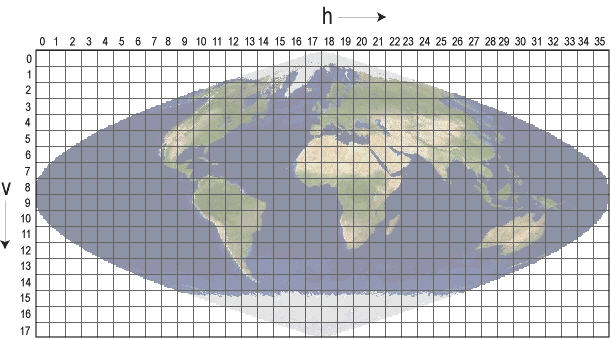
\includegraphics[scale=0.6]{./Grafiken/RefSys/modis_sinusoidal_grid.jpg}
\caption{\textit{MODIS Tilling System, (U.S.G.S., 2013)}}
\end{figure}



\subsection{UTM-Referenzsystem}
Sämtliche Daten der Landsatmissionen sind im \textit{Universal Transverse Mercator}-Referenzsystem (UTM) projiziert. Es handelt sich hierbei um ein globales Koordinatensystem das die Erdoberfläche von 80 Grad Süd bis 84 Grad Nord streifenförmig in 6 Grad breite Zonen unterteilt. Als Basis dient das Bezugsellipsoid WGS84. UTM nutzt eine transversale Mercator-Projektion zum verebnen. Hierbei berührt der Projektionszylinder die Oberfläche nicht am Bezugsmeridian sondern schneidet sie. Dadurch ensteht ein Streifen

\section{MODIS - Allgemeine Informationen zum Sensor und Trägersystem}


MODIS ( Moderate Resolution Imaging Spectroradiometer) nennt sich ein optischer Sensor, welcher sich in einem Low Earth Orbit in 705 km Höhe, mit einer Blickwinkel von 2330 km auf den beiden Satelliten Terra (früher EOS AM-1) und Aqua (früher EOS PM-1) um die Erde befindet. Die Mission wurde am 18. Dezember 1999 mit dem Launch des Terra (EOS AM-1) Spacevehicles gestartet. Am 4. Mai 2002 wurde der Satellite Aqua (EOS PM-1) mit dem zweiten MODIS in seine Umlaufbahn geschossen. Die Lebenszeit von Terra und Aqua war mit jeweils 6 Jahren anberaumt und erfreut sich nun über ein mehr als 15 jähriges Bestehen. Die Orbits der Satelliten sind so synchronisiert, dass Terra den Äquatior am Vormittag von Nord nach Süd passiert und Aqua den Äquator nachmittags von Süd nach Nord. Die räumliche Auflösung eines einzenlnen Pixels reicht von 250 und 500 Metern im Nadir bis zu 1 km als Whisk-Broom-Scanner. Die Bänder 1-2 werden in 250m, die Bänder 3-7 in 500m und die Bänder 8-37 werden in 1000m Auflösung aufgenommen. Beide Satelliten vermögen in einer ein bis zwei Tage Periode die gesamte Erdoberfläche in 36 spektralen Bändern in einem Umfang von $0.4\mu$ m bis $14.4\mu$ m aufzunehmen. Die Aufnahmen finden dabei jeweils unter einem anderen Einstrahlwinkel, bidirektional,  der Sonne statt. Nach der Anwendung von atmosphärischen Korrekturen und der Überführung der Strahlungswerten in Reflexionswerten der Erdoberfläche gibt das System die anisotropischen Reflexionseigenschaften mit dem Wandel der Landbedeckungstypen, Vegetation sowie Bodenkomponenten  in jedem einzelnen Pixel wieder. Anhand von State-of-the-Art On-board-Kalibrierungseinheiten wird eine Genauigkeit von unter 2\% angegeben (Vermote E.F., Saleous N.Z.,2006). MODIS Terra wird generell als einer der am besten kalibierten Sensoren im Bereich der "`reflektierenden"' Wellenlängen mit einer Unsicherheit von 2\% (Helder et al., 2013).
\newline

% Spektrale Tabelle
\begin{table}[!h]
\small
\hspace{-3cm}
\begin{tabular}{|l|l|l|l|l|l|l|l|l|}
\hline
BANDNAME & MODIS & nm & Landsat 7 & nm & LANDSAT 5 & nm & LANDSAT 8 & nm \\ \hline
RED   & Band 1 & 620-670   & Band 3 & 630-690     & Band 4 & 630-690   & Band 5 & 630-680 \\ \hline
NIR   & Band 2 & 841-876   & Band 4 & 750-900     & Band 4 & 760-900   & Band 5 & 845-885 \\ \hline
BLUE  & Band 3 & 459-479   & Band 1 & 450-515     & Band 1 & 450-520   & Band 2 & 450-515 \\ \hline
GREEN & Band 4 & 545-565   & Band 2 & 525-606     & Band 2 & 520-600   & Band 3 & 525-600 \\ \hline
MIR   & Band 5 & 1230-1250 & Band 6 & 1040-1250   & Band 6 & 1040-1250 & Band 9 & 1360-1390 \\ \hline
MIR   & Band 6 & 1628-1652 & Band 5 & 1550 - 1750 & Band 5 & 1550-1750 & Band 6 & 1560-1660 \\ \hline
MIR   & Band 7 & 2105-2155 & Band 7 & 2090-2350   & Band 7 & 2080-2350 & Band 7 & 2110-2300 \\ \hline
\end{tabular}
\caption{Vergleich der aufzunehmenden spekrtalen Wellenlängen Bandweise MODIS zu Landsat Satelliten}
\end{table}

% MODIS Composites
% =================

\subsection{MODIS - Compositemethoden}
Der Grundgedanke des MODIS Compositionalgorithmus ist aus einem zeitlich vordefiniertem Pool an Epochen mittels einer reflexionsbasierten BRDF (Bi-directional Reflectance Distribution Function) mit einem eingeschränktem MVC ( Maximum Value Composite) als Rückversicherung. 
\subsubsection{Maximum Value Composite}
% Maximum Value Composite wie in AVHRR-NDVI benutzt wird
Das Maximum Value Composite (MVC) Verfahren zieht aus einem zeitlich vordefiniertem Pool für den NDVI den maximalen Wert jedes Pixels und trägt ihn in die abschliessende Epoche ein. Diese Vorgehensweise ist so geschaffen um störende  atmosphärische Effekte zu minimieren , Wolken inkludiert. Der Kompositionsvorgang inkludiert in der Regel ein Wolkenscreening sowie einen Qualitätscheck der Daten. Die MVC funktioniert eher über Oberfläcgen mit Lambert'schen Eigenschaften, bei sich ändernden atmosphärischen Eigenschaften und anisotropischem Oberflächenverhalten wird die Methode jedoch ungenau (Van Leeuwen et al., 1999). Nach atmosphärischer Korrektur nimmt die Ungenauigkeit der MVC noch zu da die Anisotropie der Oberflächen ebenfalls zunimmt. Generell arbeitet die  MVC am besten bei atmosphärisch unkorregierten Daten und ist ungeeignet für die atmosphärisch korregierten Oberflächenrefelxions Daten des MODIS-Sensors. Der NDVI tendiert zu einer Zunahme nachdem er aus atmosphärisch korregierten Daten berechnet wurde, jedoch bedeutet der höchste NDVI für ein Pixel noch nicht, dass es auch um den  besten atmosphärisch korregierten Pixel handelt. Nicht entfernte Wolken und sowie unterschiedliche Sonnen- und Beobachtungswinkel verändern die Oberflächenrefelxion und somit den ausgewählten maximalen Wert. Über das Jahr gesehen wäre somit der Pixel nicht konsistent ( Van Leeuwen et al., 1999). Generell überschätzt das MVC-Verfahren die Rasterwerte und führt in weiterer Folge auch zu einer Überschätzung der abgeleiteten Parameters ( Van Leeuwen et al., 1999). Wird der NDVI nun aus atmosphörisch korregierten Daten berechnet, so sind vor allem Pixel im Off-Nadir Bereich mehr fehlerbehaftet, da hier die Korrektur nicht so gut funktioniert.
Einhergehend mit der immer weiter voranschreitenden Verbesserung und  Entwicklung der atmosphärischen Korrekturalgorithmen wird bidirektionale Reflexion an Bedeutung gewinnen, da hier die unterschiedliche Struktur der Oberflächenbedeckung mit berücksichtigt werden kann.\newline




\subsection{Datenakquisition - v5}
Die  rohen MODIS-Zeitreihe liegt als verrauschete Zeitreihe von 2000-2012 im hdf-4 Format vor und  wurden mittels der NASA-eigenen Software "`MRT-TOOL"' in das GeoTIFF-Format entpackt und in das Sinusodial Reference System transformiert. Die Zeitreihe an sich selbst, setzt sich aus 16-Tägigen Kompositionen der besten spektralen Einzelaufnahme eines Pixels zusammen. Abhängig von der Auflösung des verwendeten Produktes zum Beispiel im 250 Meter aufgelöstem Produkt kann auch zwischen den Aufnahmen des Terra Satelliten mit dem Postfix "MOD" und dem Aqua Satelliten mit dem Postfix "MYD" unterschieden werden, welches zusätzlich in der Programmierung bedacht werden muss. Aufgrund der unterschiedlichen Launchzeitpunkte der Satelliten wurde die Zeitreihe zwischen 2000 und der ersten Aqua-Aufnahme künstlich verdichtet, indem die Terra-Aufnahmen einfach verdoppelt wurden und einen passenden Zeitstempel erhalten haben. Die komplettierte Zeitreihe an sich selbst weist alle 8 Tage eine Epoche eines MODIS-Sensors (Terra und Aqua-Epochen immer abwechselnd) auf.Für die Diplomarbeit selbst beschränkt sich der Author auf das "`500m"' aufgelöste Produkt MCD43A4 welches alle 8 Tage Daten des Terra- oder des Aqua-Satelliten inklusive die passende Qualitätsinformation zur Verfügung stellt. 
Trotz des einwandfreien Rufes einer perfekten radiometrischen Korrektur der MODIS-Daten wurden Störungen in der visuellen Kontrolle ausfindig gemacht und die Zeitreihe anhand eines Glättungsalgorithmus nach Savitzky-Golay verbessert. Somit liegt eine europaweite wolkenfreie MODIS-Zeitreihe in 500 Meter Pixelauflösung als Basis für die relative Kalibrierung der Landsatdaten bereit.
% - HDF interne Struktur
% - Day of Year fertig beschreiben
\subsection{Datenakquisition - MODIS Zeitreihe V6}
%\subsection{MODIS}
%Die 500m aufgelösten MODIS-Daten sowie deren epochenzugehörige Qualitätsinformation im hdf4-Format wurden von einem mittlerweile geschlossenem FTP Server der NASA mittels einem Python FTP-Skript heruntergeladen und epochenweise lokal als hdf4-Stack verspeichert. Das hdf4-Format ist ein Containerformat welches vor allem in der wissenschaftlichen Community weit %verbreitet ist. Das Datenprodukt trägt die Kennzeichnung MCD43A4 und das zugehörige Qualitätsprodukt die Kennzeichnung MCD43A2. Aus den hdf4-Stacks wurden  mittels Python-Skript für die 500m Daten die Bänder \begin{enumerate} \item Rot \item NIR \item Blau \item Grün \item 3 mal MIR ( siehe Tabelle ) \end{enumerate} mittels dem MRT-Tool sowie aus dem Qualitätsprodukt %jener Layer mit der Qualitätsinformation der Albedo extrahiert und als GeoTIFF verspeichert. Die Rohdaten liegen nach dem Entpacken in der sinusoidalen Projektion vor.

\subsubsection{MODIS Data General Describtion}
% MODIS steht für\emph{\textbd{MOD}erater-resolution \textbf{I}maging \textbf{S}pectrometer} (MODIS)
%[1]https://ladsweb.modaps.eosdis.nasa.gov/missions-and-measurements/products/MCD43A2/
%[2]https://developers.google.com/earth-engine/datasets/catalog/MODIS_006_MCD43A2#bands
%[3]https://lpdaac.usgs.gov/products/mcd43a2v006/
%[4]https://www.umb.edu/spectralmass/terra_aqua_modis/modis_brdf_albedo_product_mcd43
%[5]https://ladsweb.modaps.eosdis.nasa.gov/missions-and-measurements/products/MOD09GA/
%[6]https://landweb.modaps.eosdis.nasa.gov/cgi-bin/QA_WWW/newPage.cgi?fileName=maturity
%[7]https://ladsweb.modaps.eosdis.nasa.gov/filespec/MODIS/6/MCD43A2
%[8]https://lpdaac.usgs.gov/products/mcd43a4v006/
%[9]https://www.umb.edu/spectralmass/terra_aqua_modis/v006/mcd34a4_nbar_product
%[10]https://e4ftl01.cr.usgs.gov/MOTA/
MCD steht für eine Kombination aus TERRA und AQUA Daten, welche für die Herstellung dieses Produktes herangezogen wurden, um die größt mögliche Güte der Qualitätsinformation zu gewährleisten. Der herangezogene Zeitraum beträgt 16 Tage und das Datum des Files repräsentiert dabei das Zentrom des Moving-16-tages-Windows [1]. Die täglichen Produkte werden hinsichtlich ihrer Qualität, Beobachtungsabdeckung und zeitlichen Distanz zum interessierenden Zeitpunkt gewichtet [4]. MCD43 Produkte verwenden L2G-lite Daten als Input [3]. Wenn zuwenige Beobachtungen vorliegen ( aus den unterschiedlichen Orbits), dann wird mit Hilfe einer Datenbank, welche urtypische BRDF Parameter enthält eine "lower-magnitude" Inversion durchgeführt und angewandt[3].
Die rohen MODIS Datenpunkte mit der Kennung MCD43A4  und den epochenweisen zugehörigen Qualitätsinformation mit der Kennung MCD43A2 liegen als HDF4 auf einem Server des United States Geological Survey (USGS) auf und können dort über die Website \footnote{https://e4ftl01.cr.usgs.gov/MOTA/} bezogen werden (eine Registrierung wird vorausgesetzt). Das HDF4 Format ist ein Containerformat das unterschiedlichste Datentypen kombiniert in einem File hierarchisch bzw multidimensional verspeichern kann. Vorteil ist vor allem bei diesem Format, dass man auch an bestehenden Dateien neue Daten anhängen kann.

\subsubsection{MCD43A4 NBAR Data} \label{NBAR}
MODIS MCD43A4 Version 6 ist ein Nadir BRDF (Bidirectional Reflectance Distribution Function) angepasstes Reflexionsprodukt (NBAR) aus ebenfalls 16 tägigen Auqa und Terra Daten. Die Daten werden für den Sonnenhöchststand der Tagesepoche berechnet [9]. Daraus resultiert ein stabiles und konsistentes NBAR Produkt. Die Daten werden mit einem überblicksartigen Qualitylayer für jedes Band in einem HDF Stack verspeichert. Es wird jedoch explizit darauf hingewiesen bei Berechnungen oder sonstiger Verwendung die Qualityinfo aus den MCD43A2 Produkten zu verwenden, da diese eine höhere Genauigkeit aufweisen. Die berechneten Reflexionswerte werden für jede Band als Rasterdaten in 16bit verspeichert. Fill value oder NoDate value ist 32767 [←8].
\subsubsection{MCD43A2 Quality Product} \label{MCD43A2_qualy_desc}
Die Beobachtungen sind auf den neunten Tag der 116 Tagesperiode gewichtet [3]. Dies führt auch zu einer besseren Qualität in höheren Breiten. Im Vergleich hierzu, Version 5 verwendet ein Fenster von nur vier Beobachtungen pro Tag [3]. Die Qualitätsinformation für die Bänder 1 - 7 befinden sich im HDF-Stack des Qualitätsproduktes in den Layern 11-17 und weisen die Qualität nach folgendem Schlüssel aus [7]
\begin{itemize}
\item 0 = best qualiy, full inversion (WoDs, RMSE majority good)
\item 1 = good quality, full inversion ( also including the cases that no clear sky observations over the day of interest or the Solar Zenith Angle is to large even WoDs, RMSE majority good)
\item 2 = Magnitude inversion ( numobs $>$=7)
\item 3 = Magnitude inversion ( 2$>$= numobs $<$7)
\item 4 = Fill value
\end{itemize}
Der Fill value ist mit 255 dem NoData Value gleichzusetzen, da er so in den Qualitätsdaten vorkommt. 
\begin{figure}[H]
\centering
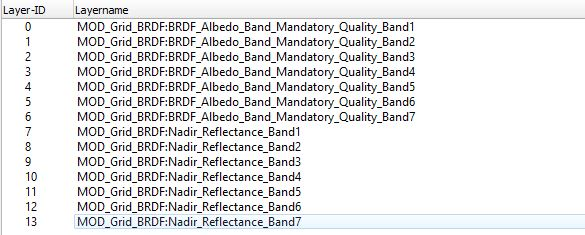
\includegraphics{./Grafiken/Datenakquisition/HDF5_MCD4A4_Layerhierarchy.JPG}
\caption{\textit{Layerhierarchie eines HDF4 Files}}
\end{figure}
In den Datenfiles sind auch Qualitätsinformationslayer enthalten, diese bieten jedoch nicht die Genauigkeit des Qualitätsproduktes MCD43A2. 
\begin{figure}[H]
   \begin{minipage}[b]{.4\linewidth} % [b] => Ausrichtung an \caption
      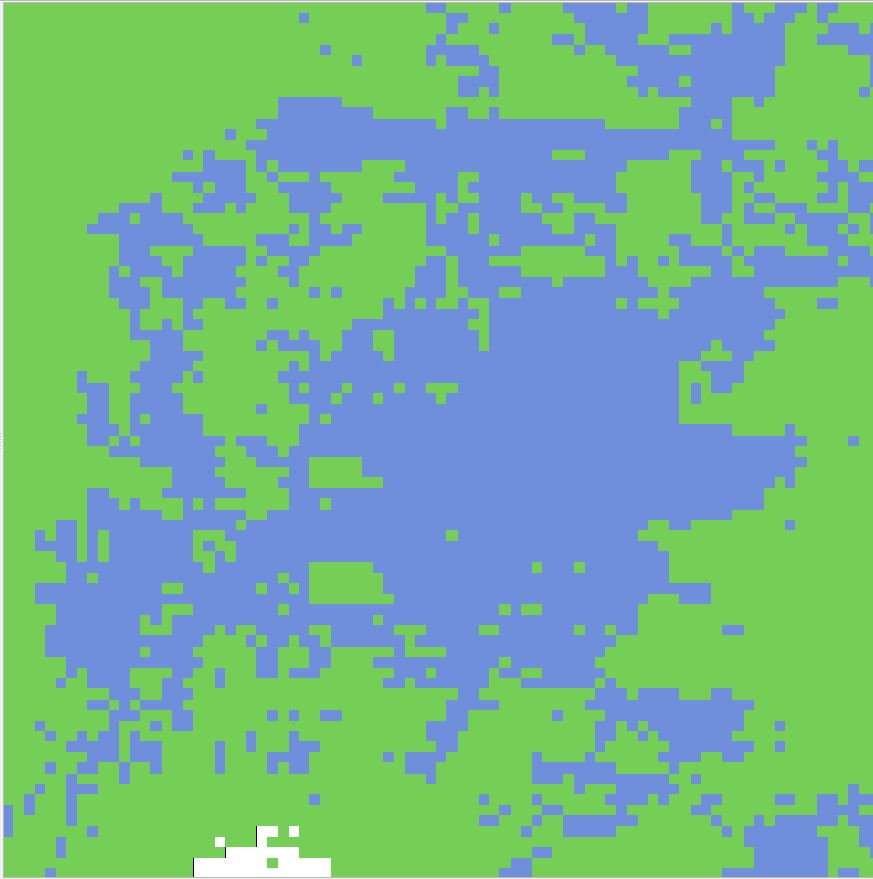
\includegraphics[width=\linewidth]{./Grafiken/Datenakquisition/Quali_verleich_MCD43A4.JPG}
      \caption{Qualitätsinformation aus dem Datenprodukt}
   \end{minipage}
   \hspace{.1\linewidth}% Abstand zwischen Bilder
   \begin{minipage}[b]{.4\linewidth} % [b] => Ausrichtung an \caption
      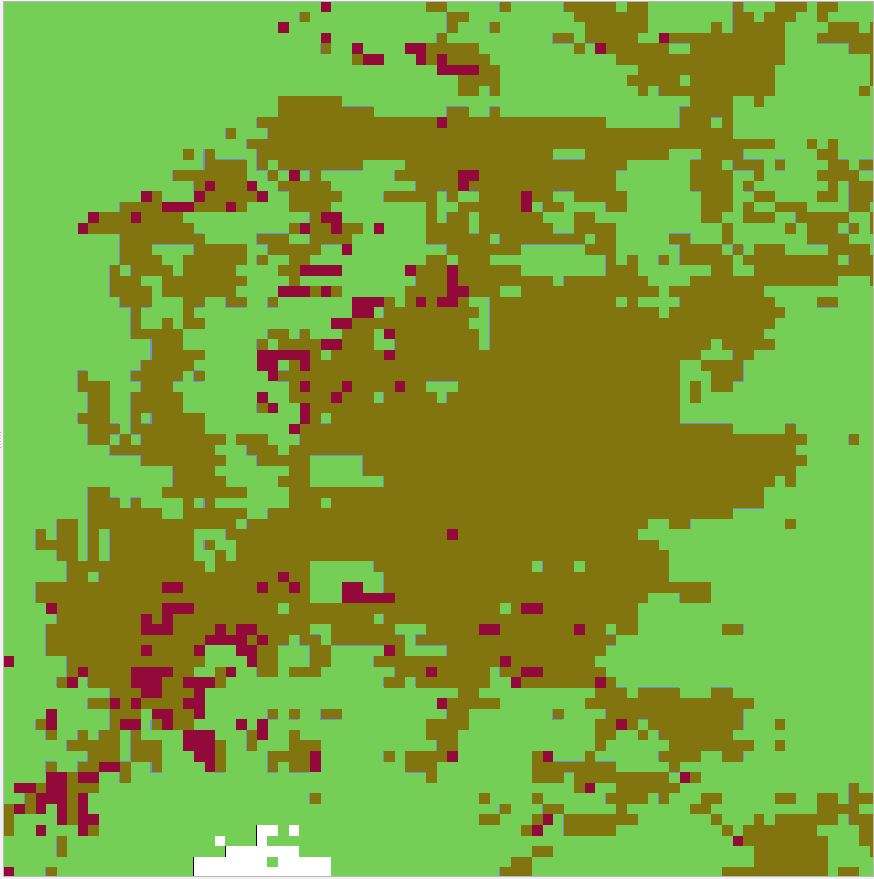
\includegraphics[width=\linewidth]{./Grafiken/Datenakquisition/Quali_verleich_MCD43A2.JPG}
      \caption{Qualitätsinformaion aus dem Qualitätsprodukt}
   \end{minipage}
\end{figure}

Der Dateiname jeder Datenepoche oder der zugehörigen Qualitätsinformation beinhaltet 
\begin{itemize}
\item Dateiname=MCD43A4.A2000057.h18v04.006.hdf 
\item Produkt = MCD43A4 (hier Datenprodukt)
\item Day Of Year = A2000057 
\item Kachel = h18v04
\item Version = 006
\item Fileextension = hdf
\end{itemize}
Um ein Jahr zu rekonstruieren bzw zu filtern werden 46 Datenpunkte verwendet. Dies entspricht den Day of Year von 001 bis 361 in einem Intervall mit an jedem 9.ten Tag einen Datenpunkt. Da es sich für den in Betracht gezogenen Zeitraum 2000-2020 um 927 Datenpunkte pro Kachel handelt, wurde hier mit Python bzw den Bibliotheken \emph{requets, bs4} ein Webscrabber-Skript geschrieben, welches alle Metadaten für die zu interessierenden Daten erstellt und aus der passenden Ordnerstruktur am USGS Server downloaded und in einer passenden Ordnerstruktur lokal verspeichert.

\begin{figure}[H]
\centering
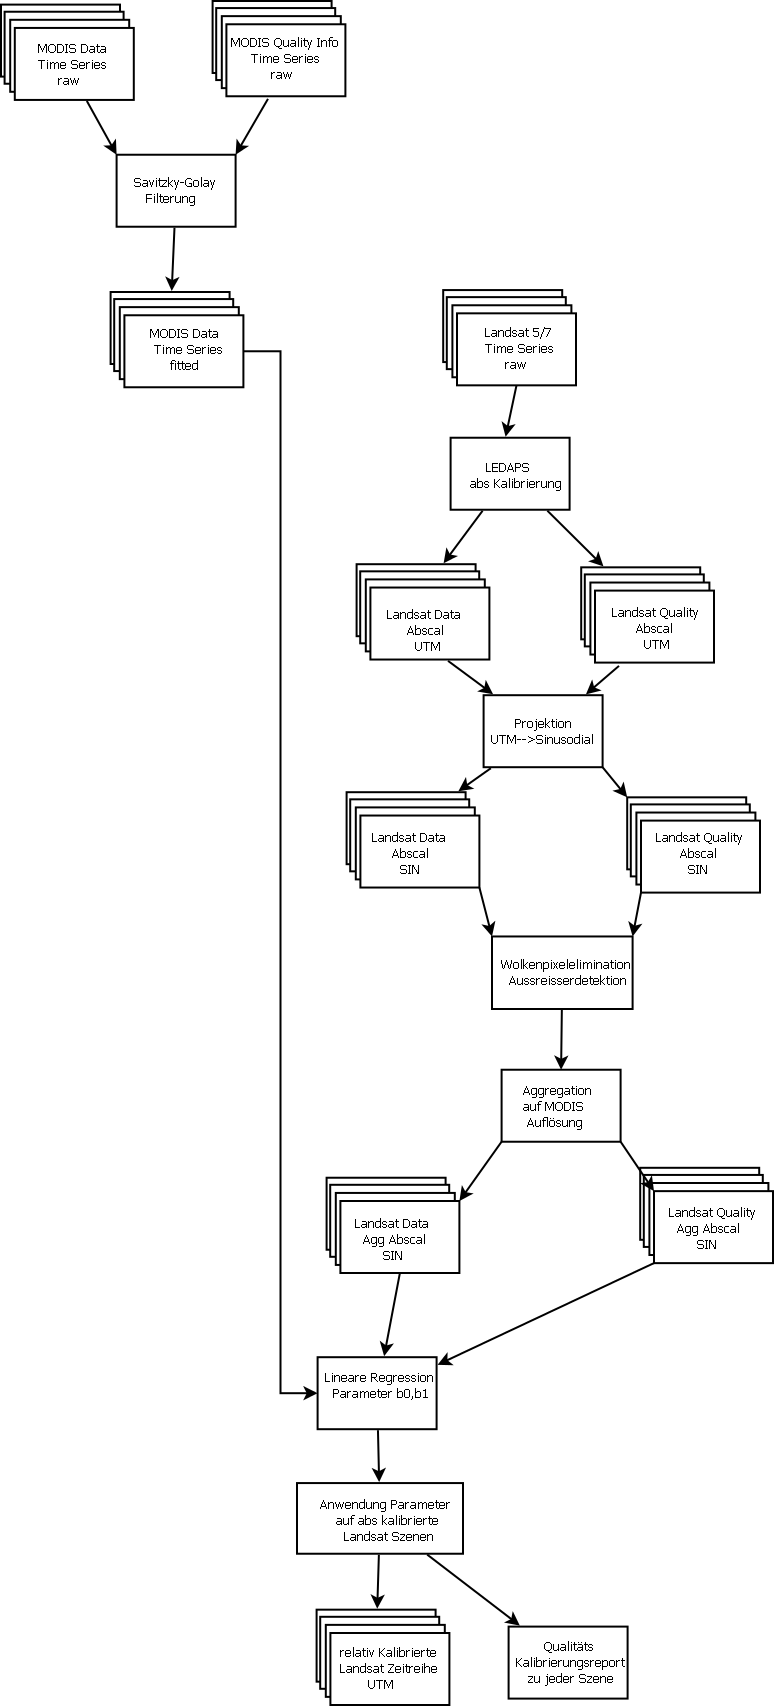
\includegraphics[width=\textwidth,height=\textheight]{./Diagramme/Workflow_rel_Kal.PNG}
\caption{\textit{Workflow der relativen Kalibrierung von Landsatdaten mittels gefilterter MODIS Zeitreihe}}
\end{figure}



% ==============================================================================================================
% METHODIK
% Mathematische Grundlagen
% 
% ==============================================================================================================

\section{mathematische Grundlagen}

Das Hauptziel der Diplomarbeit besteht darin, aus einer dichten Zeitreihe von atmosphärisch gut korrigierten MODIS-Satellitenbilddaten anhand von statistischen Methoden und Werkzeugen Landsat TM und Landsat ETM+ Satellitenbilddaten in Oberflächenreflexion überzuführen und radiometrisch zu verbessern. In diesem nachfolgenden Kapitel wird auf die mathematischen und statistischen Grundlagen eingegangen die für das Verständnis von Nöten sind. Die verwendeten Informationen stammen zumeist aus \textit{Regresison} (Härdle, 2007) sowie dem Vorlesungsskriptum aus \textit{Parameterschätzung} von (Pail, 2010).

\subsection{statistische Kennzahlen}
\begin{equation}
\bar{x}=\frac{1}{n}\sum_{i=1}^{n} x_i \qquad\qquad \dots \ Mittelwert
\end{equation}
\begin{equation}
\bar{\sigma^2}=\frac{1}{n-1}\sum_{i=1}^{n} (x_i - \bar{x})^2 \qquad \dots \ Varianz
\end{equation}
\begin{equation}
\sigma=\sqrt{\sigma^2} \qquad\qquad \dots \ Standardabweichung
\end{equation}


\subsection{Lineare Regression}
\subsubsection{OLS - das klassische lineare Modell}
% aus dem Regressionsbuch Kapitel 3

Generell gilt der Zusammenhand das $y$, die Variable die primär von Interesse ist, eine Funktion von $x_1,\dots,x_k$ ist. Allgemein wird der Zusammenhang zwischen $y$ und $x_1,\dots,x_k$ als Funktion $f(x_1,\dots,x_k)$ beschrieben. Da diese Beziehung nicht exakt gemessen werden kann wird diese Beziehung immer durch zufällige Störungen verzerrt.
\begin{equation}
y=f(x_1,\dots,x_k)+\epsilon
\end{equation}\newline
Generelles Ziel ist die Schätzung der zugrundeliegenden unbekannten Funktion $f$. Über die unbekannte Funktion $f$ und den Fehler $\epsilon$ werden folgende Annahmen getroffen:\newline
\begin{enumerate}
\item Die systematische Komponente f ist eine Linearkombination der Kovariablen\\
Anhand der Kovariablen wird die Funktion als Linearkomination modelliert.
\begin{equation}
f(x_1,\dots,x_k) = \beta_0, + \beta_1 x_1 +  \dots + \beta_k x_k
\end{equation}\\
Die Parameter $\beta_0, + \beta_1 x_1 +  \dots + \beta_k x_k $sind allesamt unbekannt und werden geschätzt, wobei $\beta_0$ als Konstante verwendet wird ( Intercept). Zusammengefasst in Vektoren mit der Dimension $p=(k+1) , x=(1,x_1,\dots,x_k)'$ und $\beta=(\beta_0,\dots,\beta_k)$ ergibt sich die kompaktere Schreibweise
\begin{equation}
f(x) = x'\beta
\end{equation}

\item Additivität der Störgröße
Die Additivität der Störgröße wird als weitere Grundanahme des linearen Modells  angenommen
\begin{equation}
f(x) = x'\beta + \epsilon
\end{equation}
Für die zu schätzenden unbekannten Parameter \textbf{$\beta$} zu den erhobenen Daten $y_i$ sowie $x=(1,x_1,\dots,x_k)', i=1,\dots,n$ existiert eine Beobachtungsgleichung für jede Beobachtung 
\begin{equation}
y_i = \beta_0 + \beta_1 x_1 +  \dots + \beta_k x_k + \epsilon_i = x_i'\beta + \epsilon_i
\end{equation}
Anhand der  Vektoren
\begin{equation}
y=\left(\begin{array}{c}y_1\\ \vdots \\ y_n \end{array} \right) \qquad sowie \qquad \epsilon = \left(\begin{array}{c}\epsilon_1\\ \vdots \\ \epsilon_n \end{array} \right)
\end{equation}
und der Designmatrix X 
\begin{equation}
P_{ij} = \left( \begin{array}{cccc} 1 & x_{11} & \ldots & x_{1k} \\ \vdots & \vdots & \ddots & \vdots \\ 1 & x_{n1} & \dots & x_{nk} \end{array} \right) = \left(\begin{array}{c}x_1' \\ \vdots \\ x_n' \end{array} \right)
\end{equation}
kann eine bequeme Matrixschreibweise angeführt werden:
\begin{equation}
y=
\end{equation}
\end{enumerate}

% Fast Fourier Transformation
% ==================================================
% verwendete Grafik 1 https://www.nti-audio.com/de/service/wissen/fast-fourier-transformation-fft
% verwendete links: benötigt für DFT O(N2) FFT O(Nlog2N) https://towardsdatascience.com/fast-fourier-transform-937926e591cb 
% 						Superpositionsprinzip Physik https://de.wikipedia.org/wiki/Superposition_(Physik) 
% Literatur Fourier Analyse - 
% - Mathematik für Ingenieure und Naturwissenschafter Band2 -  Lothar Papula - 13. Auflage 2012, S795 - da hab ich die Formal für die DFT her
% - Mathematische Methoden in der Physik - Christian B. Lang, Norbert Pucker, Kapitel 13, S 401
% 

\subsection{Harmonische Schwingungen - Fourier Analyse
}
\subsubsection{Harmonische Schwingungen , Diskrete Fourier Transformation und Analyse}
% aus Mathematische Methoden in der Physik - Christian B. Lang, Norbert Pucker, Kapitel 13, S 401, 2005
Da sich die Natur recht gut mit periodischen Funktionen beschreiben lässt, wurden auch hier einige Methoden aus der Signalanalyse und Verarbeitung gewählt um die Daten einer Zeitreihe der vorhandenen MODIS Satellitendaten zu analysieren, rekonstruieren und zu verbessern. Die Zerlegung nach Frequenzen entspricht dem, was ein Prisma mit dem einfallenden Licht macht. Der Lichtstrahl - zum Beispiel ein Sonnenstrahl - ist meist eine Überlagerung von Beiträgen verschiedenster Frequenzen. Da die Lichtbrechung beim Prisma frequenzabhängig ist, wird der Strahl zerlegt, der Ausfallwinkel hängt von der Frequenz des entsprechenden Anteils ab. Diese Zerlegung ist nichts anderes als die Projektion auf die Basisvektoren des Vektorraums periodischer Funktionen in $L^{2}$. Die Methode heißt Fourierzerlegung oder \textbf{Fourieranalyse}, die Zusammensetzung der Funktion als Summe ihrer Komponenten ist die \textbf{Fouriersynthese} (Christian B. Lang, Norbert P. 2005). 

% Grafik aus Mathemathischen Methoden in der Physik hier noch ausbessern - Prisma

\begin{figure}[H]
\centering
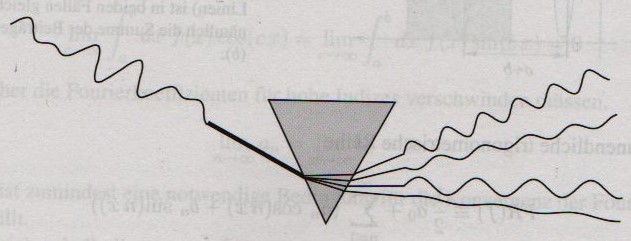
\includegraphics[scale=0.6]{./Grafiken/Fitting/FFT/prisma_cut.jpg}
\caption{\textit{Aufteilung eines Lichtstrahls in seine Frequenzbereiche (Christian B. Lang, S401)}}
\end{figure}

% Aus Mathematik für Ingenuere Band2 S 182/ 2.1 Fourier-Zerlegung
Die Daten der zu analysierenden Zeitreihe sind in der Regel keine reine sinusförmige Schwingung, besitzt jedoch ebenfalls eine Schwingungsdauer $T$ und eine Kreisfrequenz $\omega_0=2\pi / T$. Diese zeitabhängige, periodische Funktion $y(t)$ lässt sich dann unter den bekannten Voraussetzungen in eine Fourier-Reihe vom Typ

\begin{equation}\label{dft}
\begin{split}  
y(t) =\frac{a_0}{2}+\sum_{n=1}^{\infty} \lbrack a_n \cdot cos(n \omega_0 t) + b_n \cdot sin(n \omega_0 t) \rbrack = \\\
= \frac{a_0}{2}+a_1 \cdot cos(\omega_0 t) + a_2 \cdot cos(2 \omega_0 t) + a_3 \cdot cos(3 \omega_0 t) + \dots \ \\\
\dots \ + b_1 \cdot sin(\omega_0 t) + b_2 \cdot sin(2 \omega_0 t) + b_3 \cdot sin(3 \omega_0 t) + \dots\ 
\end{split}
\end{equation}
entwickeln. Diese Entwicklung in unendlich viele Sinus- und Kosinusfunktionen bedeutet aus physikalischer Sicht eine Zerlegung der Schwingung $y(t)$ in ihre harmonischen Bestandteile, auch Schwingungskomponenten genannt. Sie bestehen aus der Grundschwingung mit der Grundkreisfrequenz $\omega_0$ und den harmonischen Oberschwingungen deren Kreisfrequenzen ganzzahlige Vielfache der Grundkreisfrequenzen sind: $2\omega_0, 3\omega_0, 4\omega_0 \dots $. Bringt man umgekehrt Grundschwingungen und Oberschwingungen zur ungestörten Überlagerung, so erhaltet man als Resultierende genau die Schwingung $y = y(t)$ (Superpositionsprinzip der Physik \footnote{ungestörte Überlagerung (Interferenz) mehrerer Wellen des gleichen Typs. Hier können sich die Amplituden der (z.B. elektromagnetischen) Wellen beim Überlagern gegenseitig verstärken oder abschwächen}). Die Fourier-Koeffizienten $a_0, a_1, a_2, a_3, \dots, b_1, b_2, b_3, \dots $ bestimmen dabei die Amplituden der harmonischen Teilschwingung und somit letztendlich deren Anteile an der Gesamtschwingung (Lothar P., S182). Die als harmonische Analyse oder auch \emph{Fourier-Analyse} bezeichnete Zerlegung einer nichtsinusförmigen Schwingung $y=y(t)$ in Grundschwingung und harmonische Oberschwingungen läuft somit auf die Bestimmung der Fourier-Koeffizienten in der Entwicklung nach der vorangegangenen Formel (\ref{dft}) hinaus. 

\begin{equation}
y(t) =\frac{a_0}{2}+\sum_{n=1}^{\infty} \lbrack a_n \cdot cos(n \omega_0 t) + b_n \cdot sin(n \omega_0 t) \rbrack \\\
\end{equation}
Sie können mit Hilfe der folgenden Integralformeln berechnet werden (Lothar P., S183)
\begin{eqnarray}
\omega_0: &  & \textnormal{Kreisfrequenz der Grundschwingung} \\
n\omega_0: &  & \textnormal{Kreisfrequenz harmonischer Oberschwingungen (n=1,2,3..)} \\
T = \frac{2\pi}{\omega_0}: &  & \textnormal{Schwingungsdauer (Periode)} 
\end{eqnarray}
\begin{eqnarray}
a_0 = & & \frac{2}{T} \cdot \int_{T} y(t) dt 
\end{eqnarray}
\begin{eqnarray}
a_1 = & & \frac{2}{T} \cdot \int_{T} y(t) \cdot cos(n\omega_0t)dt \dots n=1,2,3,...  
\end{eqnarray}
\begin{eqnarray}
a_2 = & & \frac{2}{T} \cdot \int_{T} y(t) \cdot sin(n\omega_0t)dt \dots n=1,2,3,... 
\end{eqnarray}
Das Symbol $T$ im Integral bedeutet, dass die Integration über ein beliebiges Periodenintervall von der Länge T zu erstrecken ist. Die Berechnung des Koeffizienten $a_0$ ist auch mit der Formel für $n=0$ möglich, da $cos(0\omega_0t)=cos0=1$ ist(Lothar P., 2013, S183).


Die Fourier-Analyse einer nicht-sinusförmigen Schwingung $y=y(t)$ lässt sich auch in komplexer Form vornehmen:
\begin{equation}
y(t)=\sum_{n=-\infty}^{\infty} c_n \cdot e^{jn\omega_0t}
\end{equation}
Die Berechnung der komplexen Fourierkoeffizienten $c_n$ erfolgt mit der Integralformel
\begin{equation}
c_n = \frac{1}{T} \cdot \int_{0}^{T} y(t) \cdot e^{-jn\omega_0t}dt  \\\
\end{equation}
Wobei $\omega_0$ und $T$ wieder wie folgt sich zusammen setzen
\begin{eqnarray}
\omega_0 &:& \textnormal{Kreisfrequenz der Schwingung}  \\
T & : & \textnormal{Schwingungs- oder Periodendauer} (T=2\pi/\omega_0)
\end{eqnarray}
% aus Lothar P. S 178
Die Umrechnung zwischen den reellen und der komplexen Darstellung erfolgt über folgende Gleichungen:
\begin{eqnarray}
c_0=\frac{1}{2}a_0,&c_n=\frac{1}{2}(a_n -jb_n), & c_{-n}=c^{*}_{n}=\frac{1}{2}(a_n+jb_n)
\end{eqnarray}
Die Umrechnung komplexer zur reellen Form passiert wie folgt: 
\begin{equation}
a_0=2c_0 \qquad a_n=c_n+c_{-n}= c_n + c^{*}_{n} 
\end{equation}
\begin{equation}
b_n=j(c_n-c_{-n})=j(c_n - c^{*}_{n})
\end{equation}

% vielleicht in die Durchführung reinpacken?
\subsubsection{Rekonstruktion mittels FFT}
% das war aus Wikipedia
Die Fast Fourier Transformation (FFT) is eine wichtige und bekannte Methodik aus der Signalverarbeitung, welche ein Signal in ihre einzelnen Spektralkomponenten zerlegt und Aufschluss über deren Zusammensetzung gibt, Der Kern einer FFT ist eine Diskrete Fourier Transformation (DFT), jedoch ist der dahinterliegende Algorithmus optimiert, wovon auch der der Namen herrührt, sprich man verwendet die FFT um die Koeffizienten einer DFT zu ermitteln. Die FFT reduziert die Anzahl der Berechnungen für eine Anzahl \textbf{N} erheblichst
\begin{equation}
%\begin{split}
\begin{aligned}
n &= 44000\\\
DFT &= O(N^{2}) = O(44000^2) = 1 963 000 000 \\\
FFT &= O(N\cdot log_2(N)) = O(4400\cdot log_2(44000)) = 204311
%\end{split}
\end{aligned}
\end{equation}
Dies merkt man besonders wenn man große Mengen an Daten verarbeitet. Wie vorhin schon erwähnt ist die Fourier Transformation eine mathematische Operation, welche die Domäne der Zeit eines Signals in die Frequenzdomäne überführt, sprich in seine Frequenzanteile zerlegt und dadurch analysiert werden können. Bei der FFT wird ein zeitlich begrenztes Signal herangezogen und in seine Frequenzanteile zerlegt sowie deren Phasen und Amplituden bestimmt. In der Praxis wurde auf die bereits existierenden Routinen in \textbf{numpy 1.19.2} zurück gegriffen.
\begin{figure}[H]
\centering
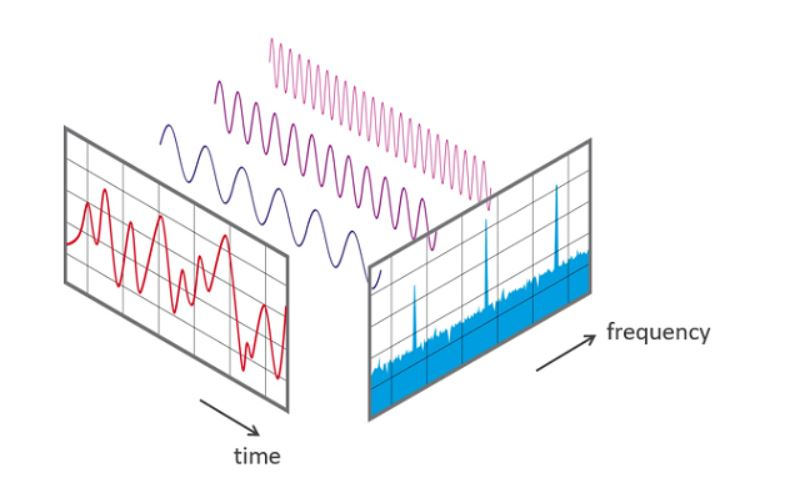
\includegraphics[scale=0.6]{./Grafiken/Fitting/FFT/FFT_time_und_frequenz_anteile.jpg}
\caption{\textit{Aufteilung eines Signals in Zeit- und Frequenzbereich}}
\end{figure}

\begin{equation}
\hat{x_k}=\sum_{i=1}^{n-1} x_i \qquad\qquad \dots \ FFT
\end{equation}



Bei genauerer Betrachtung des MODIS Datenmaterials stellt man fest, dass der Idealzustand bzw die optimalen Vorraussetzungen bei der Berechnung der Reflexionswerte eher selten vorhanden sind. Dies äussert sich als schlechtere Pixelqualitätsinformation oder gar ein nichtvorhandener Wert der durch einen Füllwert repräsentiert wird. Die FFT ist jedoch ein sehr robuster Algorithmus der auch sehr gut bei verrauschten Signalen die wichtigsten Frequenzen heraus filtert. Voraussetzung für eine erfolgreiche Analyse ist jedoch ein lückenloses Signal. Wenn nun Datenlücken aufgetreten sind, wurden diese von den vorangegangenem und dem nachfolgendem Wert linear interpoliert um einen vollbesetzten Datenarray für die Ableitung der Parameter verwenden zu können. 


% Savitzky - Golay Filterung
% ==================================================
\subsection{Anwendung Savitzky-Golay Filterung}

\subsubsection{Polynom 2. Grades}
Durch den Fakt, dass die MODIS Daten fehlerbehaftet sind, wird der Rohdatenwert durch einen gefilterten ersetzt. Um die verrauschte MODIS Zeitreihe für die später folgende relative radiometrische Kalibrierung zu filtern wurde die Methode nach Savitzky-Golay gewählt. Sie stammt aus der Signalverarbeitung und beschreibt einen Glättungsalgorithmus, der die Koeffizienten eines dem Datenmaterial zu Grunde liegend höheren Polynoms schätzt. 
Im Falle der Datenvorverarbeitung wurde ein Polynom 2. Grades gewählt, 

\begin{equation}
\label{form_poly_2nd}
f(t) = a_0+a_1 \cdot t+a_2 \cdot t^2
\end{equation}

das sich auf Werte von 15 Epochen angleicht. Dieses Fenster bewegt sich nun über den ausgewählten Datenbereich und filtert die Daten anhand des ausgewählten Polynoms. Vorteile ergeben sich daraus, dass im Vergleich zu einem gleitenden Mittel die Spitzen nicht abgeschnitten werden sondern in die Charakteristik des Polynoms mit einfließen. Nachteil sind, das nicht identifizierte Ausreißer ebenfalls so mit in die Berechnung einfließen und Einfluss nehmen. Der Wert in der Mitte des sich über die Zeit bewegenden Fensters ist im Interessenmittelpunkt und wird als später zu verwendender Wert in ein neues Rasterfile geschrieben.

Die Anzahl der Datenwerte auf der linken Seite werden als $n_L$, sowie die Datenwerte auf der rechten Seite mit $n_R$ beschrieben, wobei gilt $n_L = n_R$.
Die Parameter für das Polynom 2. Grades $M$ von $i$ , $a_0+a_1i+\dots+a_Mi^M$ werden mittels der Methode Ausgleich nach Parametern für die Werte $l_{-n_L},\dots,l_{n_R}$ bestimmt. Die Designmatrix $A$ setzte sich hierbei wie folgt zusammen:
\begin{equation}
A_{ij} = i^j\quad i = -n_L, \dots, n_R,\quad j =0,\dots,M
\end{equation}
Der Normalgleichung ausgedrückt durch den Parametervektor $\widehat{\textbf{x}}$ und dem Beobachtungsvektor \textbf{$l_i$} in Matrizenschreibweise lautet

\begin{equation}
\left(\textbf{A}^T\cdot\textbf{A}\right)\cdot\widehat{\textbf{x}}=\textbf{A}^T\cdot\textbf{l}\qquad or  \widehat{\textbf{x}}=\left(\textbf{A}^T\cdot\textbf{A}\right)^{-1}\cdot\left(\textbf{A}^T\cdot\textbf{l}\right)
\end{equation}\newline

%\begin{equation}
%A  = \left[ \frac{\partial f(t)}{\partial a_0},\frac{\partial f(t)}{\partial a_1},\frac{\partial f(t)}{\partial a_2} \right]
%\end{equation}

Anhand der Qualitätsinformation aus den MODIS-Epochen wird die Gewichtsmatrix P aufgestellt:
\begin{equation}
P_{ij} = \left[ \begin{array}{cccc} p_{11} & 0 & \ldots \\0 & p_{22} & \ldots \\ \vdots & \vdots & \ddots \end{array} \right]
\end{equation}\newline
Somit ergibt sich mit der Gewichtsmatrix folgende Form für die Normalgleichungen für den Parametervektor und den Beobachtungsvektor:

\begin{equation}
\left(\textbf{A}^T\cdot\textbf{P}\cdot\textbf{A}\right)\cdot\widehat{\textbf{x}}=\textbf{A}^T\cdot\textbf{P}\cdot\textbf{l}\qquad or \qquad \widehat{\textbf{x}}=\left(\textbf{A}^T\cdot\textbf{P}\cdot\textbf{A}\right)^{-1}\cdot\left(\textbf{A}^T\cdot\textbf{P}\cdot\textbf{l}\right)
\end{equation}\newline

Die ausgeglichenen, gefitteten Beobachtungen erhält man anhand von

\begin{equation}
\widehat{\textbf{l}} = \textbf{A}\cdot\widehat{\textbf{x}}
\end{equation}\newline

Da die Qualitätsinformation der MODIS-Epochen nicht immer ganz der Richtigkeit entsprechen ( Restwolkenpixel, Dunst etc) wird eine zweite Iteration durchgeführt und die Daten werden anhand des Verbesserungsvektors neu gewichtet:

\begin{equation}
v=-\left[ \textbf{I}-\textbf{A}\cdot\left(\textbf{A}^T\cdot\textbf{P}\cdot\textbf{A}\right)^{-1}\cdot\left(\textbf{A}^T\cdot\textbf{P}\right)   \right]\cdot\textbf{l}
\end{equation}\newline
\begin{equation}
dv=\frac{1}{v}
\end{equation}
\begin{equation}
P=\textbf{I}\cdot dv
\end{equation}\newline

\subsubsection{Gapfilling}
Da es jahreszeitenabhängig zu länger anhaltender Wolkenbedeckung und somit zu Datenlücken für die Schätzung der Parameter des Polynoms kommen kann wird anstatt des Polynoms eine Gerade verwendet. Wenn die Anzahl der Elemente linksseitig und rechtsseitig eine gewisse Mindestanzahl unterschreiten, zum Beispiel $n_L \leq 3$ und $n_r \leq 3$ so wird anstatt eines Polynom 2. Grades eine Gerade durch die Daten gelegt und der zentrale Wert der neuen Berechnung als neuer Pixelwert verwendet. Die Identifikation der zu kleinen Anzahl erfolgt durch vordefinierte Pythonroutinen.

\begin{equation}
f(t) = a_0 + a_1 \cdot t
\end{equation}\newline

Die linear zu fittenden Daten werden mittels einer Pythonroutine ermittelt und zu einem Array zusammengefügt. $n_C$ repräsentiert hierbei den eigentlich zu fittenden Wert um jenen herum normal das Polynom 2. Grades gelegt wird.
\begin{equation}
l_{ids} = l[n_L\leq 3;n_C=0;n_R\leq3]
\end{equation}\newline

Die Designmatrix bezieht sich hierbei nur auf die speziellen Situationen und variiert in ihrer Zeilenanzahl. Sie ist in ihrer Spaltenanzahl auf die Geradengleichung angepasst. Die Gewichtsmatrix verwendet jene Gewichte die bereits in der zweiten Iteration berechnet wurden. Der Beobachtungsvektor weist die gleiche Zeilenanzahl wie die Designmatrix auf
\begin{equation}
\widehat{\textbf{x}} = \left(\textbf{A}^T\cdot\textbf{P}\cdot\textbf{A}\right)^{-1}\cdot\left(\textbf{A}^T\cdot\textbf{P}\cdot\l_{ids}\right)
\end{equation}\newline

Ist der interpolierte Wert nun jedoch kleiner als das Minimum oder größer als das Maximum im Beobachtungsvektor so wird der jeweilige Maximum oder Minimumwert gesetzt.

\subsubsection{Verspeicherung der Zeitreihe}
Der Filtervorgang findet Bandweise statt. Die gefilterten Daten werden zuerst als GeoTIFF verspeichert und in einem Folgeschritt zu europaweiten Mosaicen zusammengefügt sowie epochenweise in Stacks verspeichert. Als Ergebnis liegt nun einen geglättetete, wolkenfreie Zeitreihe der MODIS-Sensoren für ganz Europa (ausgenommen Island) vor, welche zur radiometrischen Kalibrierung für Landsat5 und Landsat 7 Daten verwendet werden kann.


\subsection{Ausreisserdetektion}
Aussreissertests werden dazu benutzt um die Zuverlässigkeit von Daten zu überprüfen und vor allem extreme Erscheinungen in den Daten zu identifizieren und gegebenenfalls zu eliminieren. Ausreisser sind extrem hohe oder niedrige Werte in einer ansonst mäßig unterschiedlichen Messreihe. Im folgenden wird die Methode nach Grubbs beschrieben, welche in dieser Diplomarbeit Verwendung gefunden hat. Ziel der implementierten Ausreisserdedektion ist es vor der Aggregierung der LandsatDaten auf die MODIS-Pixel-Auflösung nicht ausmaskierte Wolkenpixel aufgrund der nicht perfekten Wolkenmaske des LEDAPS-Programmes zu identifizieren und zu eliminieren. Dies impliziert das nach extrem hohen Werten in den Daten gesucht wird. \newline

Das Verfahren selbst prüft eine berechnete Testgröße $G$ anhand des Mittelwert $\hat{x}$ und der Standardabweichung $\sigma$ des Samples und prüft ob die Hypothese oder Gegenhypothese wahr ist, das es sich bei der Beobachtung um einen Aussreisser handelt. \newline
\begin{equation}
G=\frac{max\left|x_i - \hat{x}\right|}{\sigma}
\end{equation}\newline
\begin{equation}
\alpha \qquad \dots Signifikanzniveau
\end{equation}\newline
\begin{equation}
G> \frac{(N-1)}{\sqrt{N}}\sqrt{\frac{(t_{\alpha / (2N),N-2})^2}{N-2+(t_{\alpha / (2N),N-2})^2}}
\end{equation}\newline
Viele statistische Methoden werden durch das Vorhandensein von Aussreisern beeinflusst  Bei schon simplen Berechnungen wie dem Mittelwert oder der Standardabweichung kann es zu einer Strörung durch einen einzigen "`verfälschten"` Wert kommen.

\section{Verwendete Sprachen und Programme aus dem Bereich Data Science sowie Geoinformatik}
\subsection{Softwareentwicklung mit Python}

Python ist wenn nicht die am meisten verwendete Sprache wenn es um Datenmanipulation geht. Sei es serverseitig im Backendbereich von Webservices oder Machine Learning Anwendungen, Python bietet so ziemlich zu jeder Problemstellung eine passende Herangehensweise oder Lösung. Die Community ist riesig und man findet sehr schnell Hilfe zu Problemstellungen in diversen Foren wie \emph{www.stackoverflow.com}. Im Zuge dieser Diplomarbeit wurden zwei Versionen von Python verwendet (Python 3.8 und Python 2.7) um Datenmanipulationsschritte zu automatisieren. Der gesamte Prozess der Datenakquisition, Datenaufbereitung als auch jener der relativen Kalibrierung und Ergebnispräsentation ist entweder mit bereits vorhandenen Bibliotheken oder selbstgeschrieben Modulen in Python umgesetzt worden und umfasst einige tausende Zeilen Code. Die von mir verwendete IDE zur Erstellung der Skripts und Software stammt von Jetbrains und ist unter dem Namen PyCharm sehr bekannt. Hier sei darauf hingewiesen, dass das Thema dieser Diplomarbeit sich nicht im Detail mit Problemstellungen aus der Softwareentwicklung auseinandersetzt, sondern die Softwareentwicklung mit Python als Mittel zum Zweck verwendet. Nichts destotrotz sind ein paar verwendete Feinheiten beschrieben, die einen Geschwindigkeitsvorteil in der Berechnung oder bei der Manipulation der Daten gebracht haben. 
% - Datenakquisition genauer beschreiben in einem eigenen Kapitel
\subsubsection{Python 3.8}
Python 3.8 war das Mittel zum Zweck für so ziemlich alle Arbeitsschritte um bis einschliesslich zur gefiltereten MODIS-Zeitreihe zu gelangen. Die MODIS Daten wurden mittels einem Webscrabber-Script unter Verwendung von \emph{bs4} und dem Pythoninternen \emph{requests} Modul von den NASA Servern gedownloaded, mittels \emph{GDAL} vom HDF5-Format in einzelne, bandweise GEOTIFFS konvertiert und anschliessend mittels \emph{numpy} und den vorhin beschrieben Algorithmen gefiltert oder rekonstruiert. Diese gefilterten Daten wurden weiters zu epochenweisen Stacks verarbeitet, da die relative Kalibration diese voraussetzt.
\subsubsection{Python 3.8 - Multiprocessing}
Da nur die gedownloadeten HDFS und rohen GEOTIFF Daten alleine fast einen ganzen Terabyte an Speicherplatz benötigen, war klar das es nicht sinnvoll sein kann, einem einzigen Pythonprozess die ganze Arbeit machen zu lassen. Multithreading ist am Papier mit Python möglich, aber auf Grund des Global Interpreter Locks immer an eine CPU gebunden. Paralleles Ausführen von Arbeitsschritten auf meherern CPUs ist aber mittels dem in Python integrierten Multiprocessing Modul und seit der Python Version 3.8 auch mit einem Shared Memory oder gemeinsamen Arbeitsspeicherbereich möglich. Dies erlaubt einen Speicherbereich zwischen mehreren Python Prozessen zu teilen bzw zugreifbar zu machen, um große Datenmengen parallel zu verarbeiten. Jedoch sei hier darauf hingewiesen, dass man bei der Verwendung von Shared-Memory-Objekten sich nicht mehr auf die gewohnte Typesicherheit von Python verlassen darf und zusätzlich bedenken muss: 
\begin{itemize}
\item welchen Typ hat das Shared-Memory-Objekt: -z.B. int16
\item welcher Typ kommt bei der Berechnung heraus - z.B. float64
\item in welchen Typ muss ich das Ergebnis wieder umwandeln um es am Shared-Memory-Object zu verspeichern
\end{itemize}
Wenn man dies nicht berücksichtigt kann dies es zu unerwartetem Verhalten führen und in elendslange Fehlersuche münden. Behirnt man dies jedoch korrekt, ist echtes paralleles Programmieren mit Python für CPU intensive Rechenoperationen vollumfänglich möglich.
\subsubsection{Python 2.7}
Die Rechenschritte der relativen Kalibration wurden alle in Python 2.7 getätigt. Grund waren die anfänglich verwendeten Module der arcpy API von ESRI, welche jedoch oft erhebliche Performanceprobleme hatten und im Endeffekt alle durch selbstgeschriebene Module oder durch Verwendung von bekannten Open Source Bibliotheken wie GDAL, numpy oder scipy ersetzt wurden.

\subsubsection{Anaconda}
Um zwischen den Interpreterversionen ohne Probleme hin und her wechseln zu können, wurde der Package und Virtual-Environment Manager Anaconda verwendet. PyCharm unterstützt auch unterschiedliche Interpreter die man sich als extra Runtime-Konfiguration in seinem Projekt erstellen kann.
\subsection{ArcGIS, QGIS}
Die abgeleiteten Daten benötigen natürlich eine menschliche, visuelle Kontrolle. Dies geschah in erster Linie mit ESRI's ArcMap 10.2 oder QGis 3.16. Wie schon vorhin erwähnt, wurde anfangs auch Skripts oder Toolboxen von ArcMap verwendet, jedoch durch eigene Softwaremodule ersetzt. Besonders nützlich war in beiden Programmen der Information Cursor, welcher erlaubt einzelne Pixel-Zeitreihen auf schnelle Art und Weise tabellarisch zu visualisieren und zu vergleichen. 

\subsection{Betriebsysteme, Speicherplatz und Rechenlogistik}
Hier möchte ich nur kurz Anreißen, dass die großen Datenmengen eine eigene Denkweise, Infrastruktur und Logistik erfordert haben.
Die verwendeten Betriebssysteme unterscheiden sich erheblich in den Ausführzeiten der Python Programme welche für das Rekonstruieren der MODIS Zeitreihen verwendet wurden. Deshalb wurde beim Fitten und Filtern der Daten auf Linux (Debian 10, Ubuntu 18.04) vertraut. Es kamen bis zu vier Rechner mit mindestens 4 CPUs ab 3GHz Takt und mindestens 32GB RAM zum Einsatz um die Daten parallel zu verarbeiten. Pro Spektralband der MODIS Zeitreihe kann man für 20 Jahre und jeden 9ten Tag eine vorhandene Szene ( oder 927 Datenpunkte) ca 17h Rechenzeit für Savitzky-Golay-Filter einplanen, die FFT brauchte hingegen nur an die drei Stunden. Der verbrauchte Speicherplatz für die MODIS Daten in der Version 6 sowie der Landsat Daten in roher als auch absolut Kalibrierter Form belaufen sich auf 2,42 TB (Terabyte). Um die Daten zu sichern wurde Speicherplatz im Gesamt Volumen von 11 TB angeschafft um sie auf drei unabhängigen Speichervolumen zu sichern. 

\chapter{Durchführung}
\section{Rekonstruktion und Filtern der Verrauschten MODIS V6 Zeitreihe}
Die Daten der MODIS Zeitreihe liegen mit einer Qualitätsinformation wie schon in Kapitel \ref{NBAR} beschrieben vor. Zu jedem Zeitpunkt bzw zu jedem Pixel ist nun eine Qualitätsinformation vorhanden die in der P-Matrix der Ausgleichsfunktion als Gewichtung an die Beobachtungen angebracht wird. Um einen vielfältigen Vergleich zu erhalten, welche Gewichtung die besten Resultate liefert, oder eventuell welche Tradeoffs in Kauf genommen werden müssen, wurden mehrere Iterationen der SG Filterungen mit unterschiedlicher Gewichtung vorgenommen ( dies kostet einiges an Speicherplatz!). Auch die Berechnungen der DFT wurde mit unterschiedlichen Gewichten durchgeführt, aber immer mit einer harmonischen Schwingung die auf 3 Elemente ( hat sich als als am Idealsten herausgestellt) beschränkt war. Allein die Rekonstruktion und Filterung der FFT kommt gänzlich ohne Gewichtung aus. Zu Beginn eines Jahres liegen für gewöhnlich Daten mit schlechter räumliche und temporaler Abdeckung vor, da dies vor allem mit der vermehrten Wolkenbedeckung rückzuschließen ist, siehe Abbildung \ref{MODIS_data_jan} und Abbildung \ref{MODIS_qual_jan}.

\begin{figure}[H]
   \begin{minipage}[b]{.4\linewidth} % [b] => Ausrichtung an \caption
      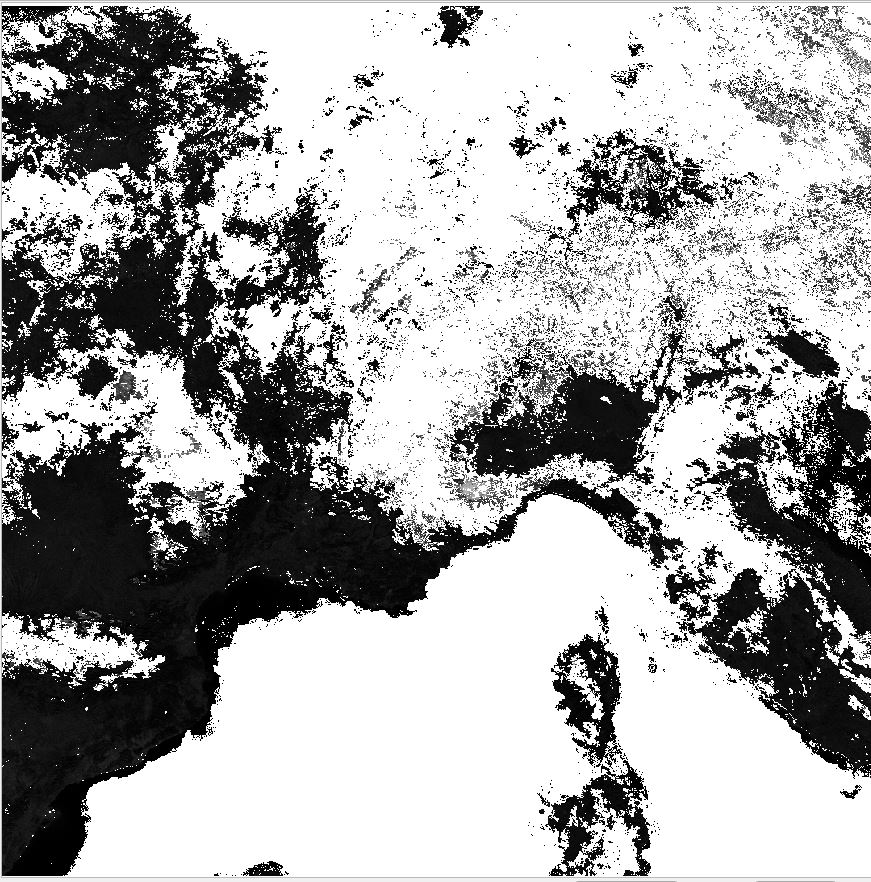
\includegraphics[scale=0.28]{./Grafiken/Fitting/Fitting_durchführung/Fitting_Vergleich_Rohdaten_Qualität_full_2.JPG}
	\caption{\textit{Bildinformation für die Kachel h18v04 für den DOY 001 des Jahres 2001 - Weiss : NoData - Graustufen: Reflexionswerte}}
   \end{minipage}
   \hspace{.1\linewidth}% Abstand zwischen Bilder
   \begin{minipage}[b]{.4\linewidth} % [b] => Ausrichtung an \caption
      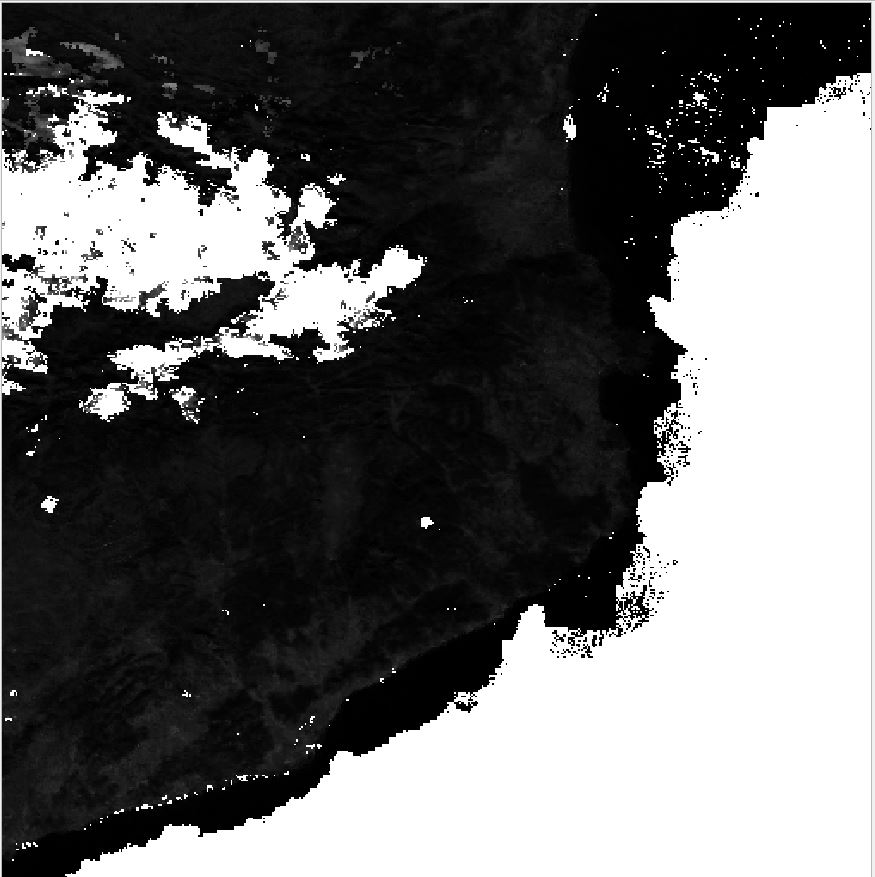
\includegraphics[scale=0.28]{./Grafiken/Fitting/Fitting_durchführung/Fitting_Vergleich_Rohdaten_Qualität_2.JPG}
\caption{\textit{Bildinformation für die Kachel h18v04 für den DOY 001 des Jahres 2001 - Weiss : NoData - Graustufen: Reflexionswerte}}
   \end{minipage}
\end{figure}

\begin{figure}[H]
   \begin{minipage}[b]{.4\linewidth} % [b] => Ausrichtung an \caption
      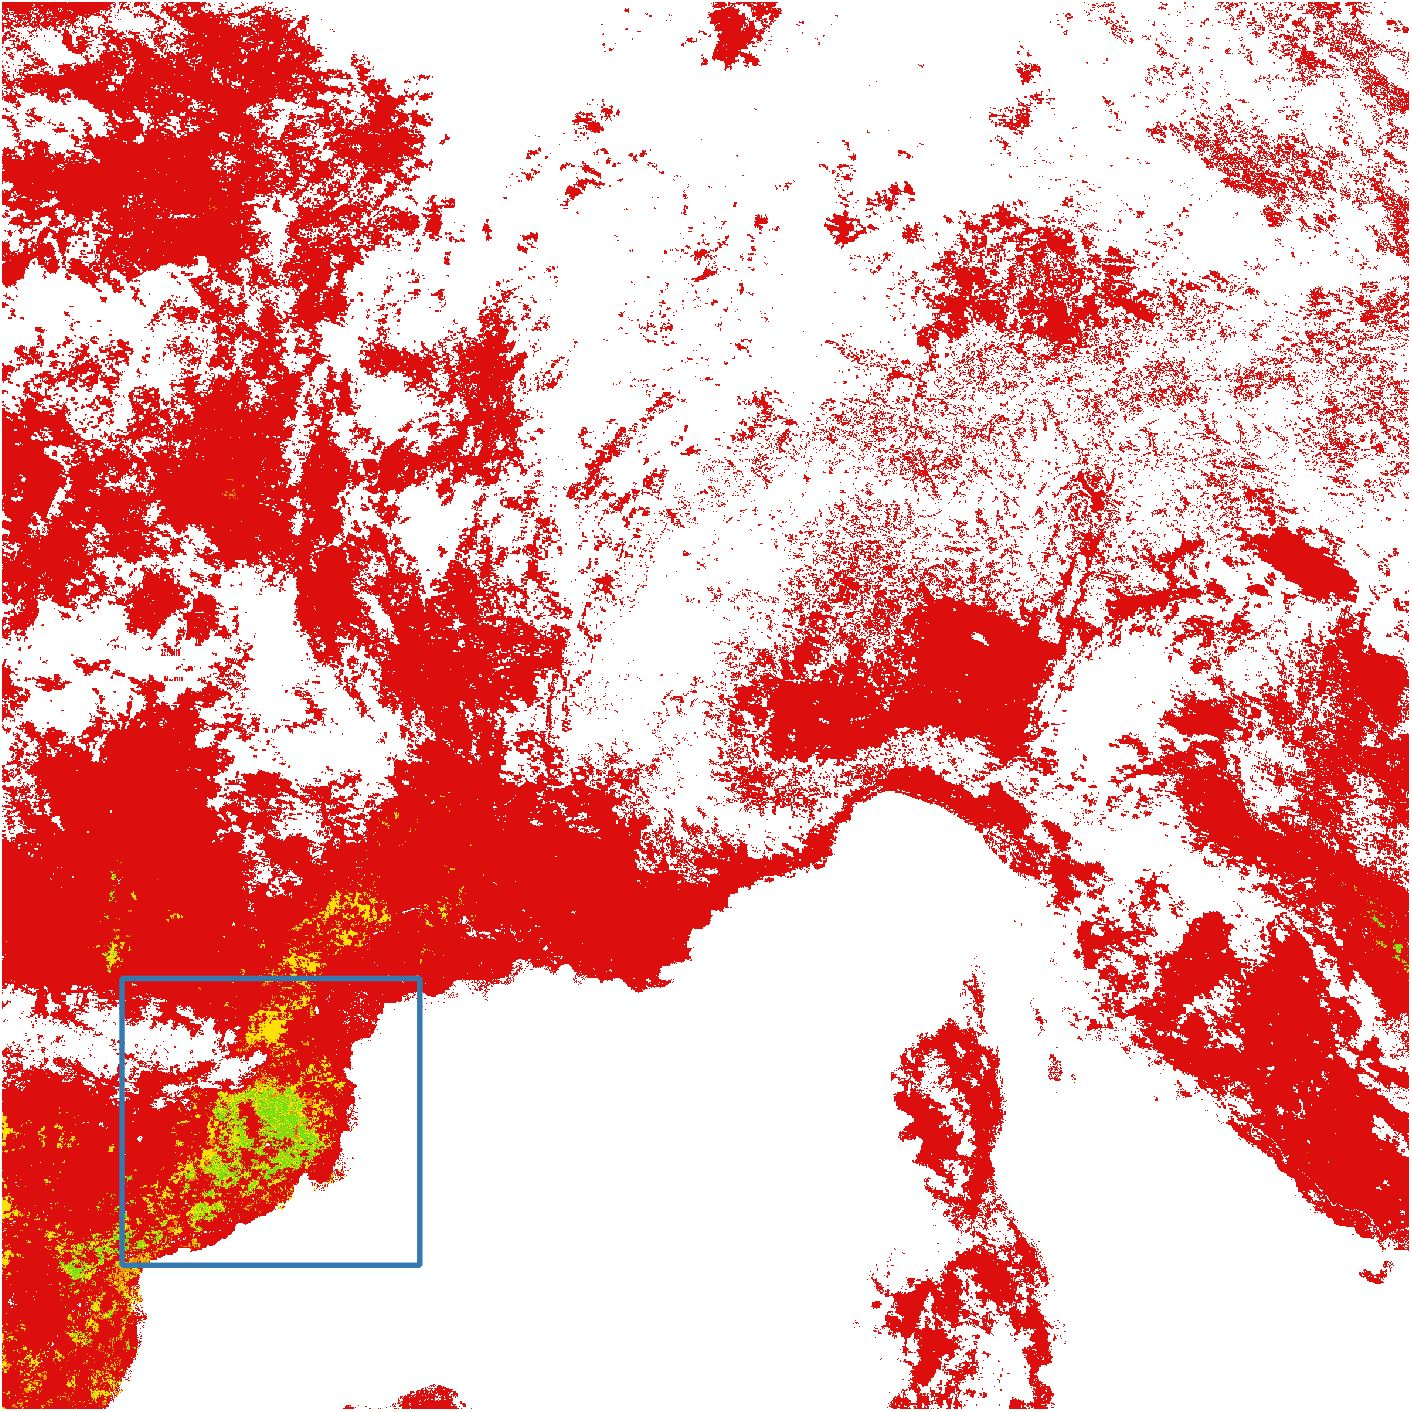
\includegraphics[scale=0.3]{./Grafiken/Fitting/Fitting_durchführung/Fitting_Vergleich_Rohdaten_Qualität_full_1.JPG}
	\caption{\textit{Qualitätsinformtion für die Kachel h18v04 für den DOY 001 des Jahres 2001 - grün: full inversion - gelb: full inversion - orange: magnitude inversion ( numobs $>$=7)  - red: magnitude inversion ( numobs $2>$=7) - white: NoData}}
   \end{minipage}
   \hspace{.1\linewidth}% Abstand zwischen Bilder
   \begin{minipage}[b]{.4\linewidth} % [b] => Ausrichtung an \caption
      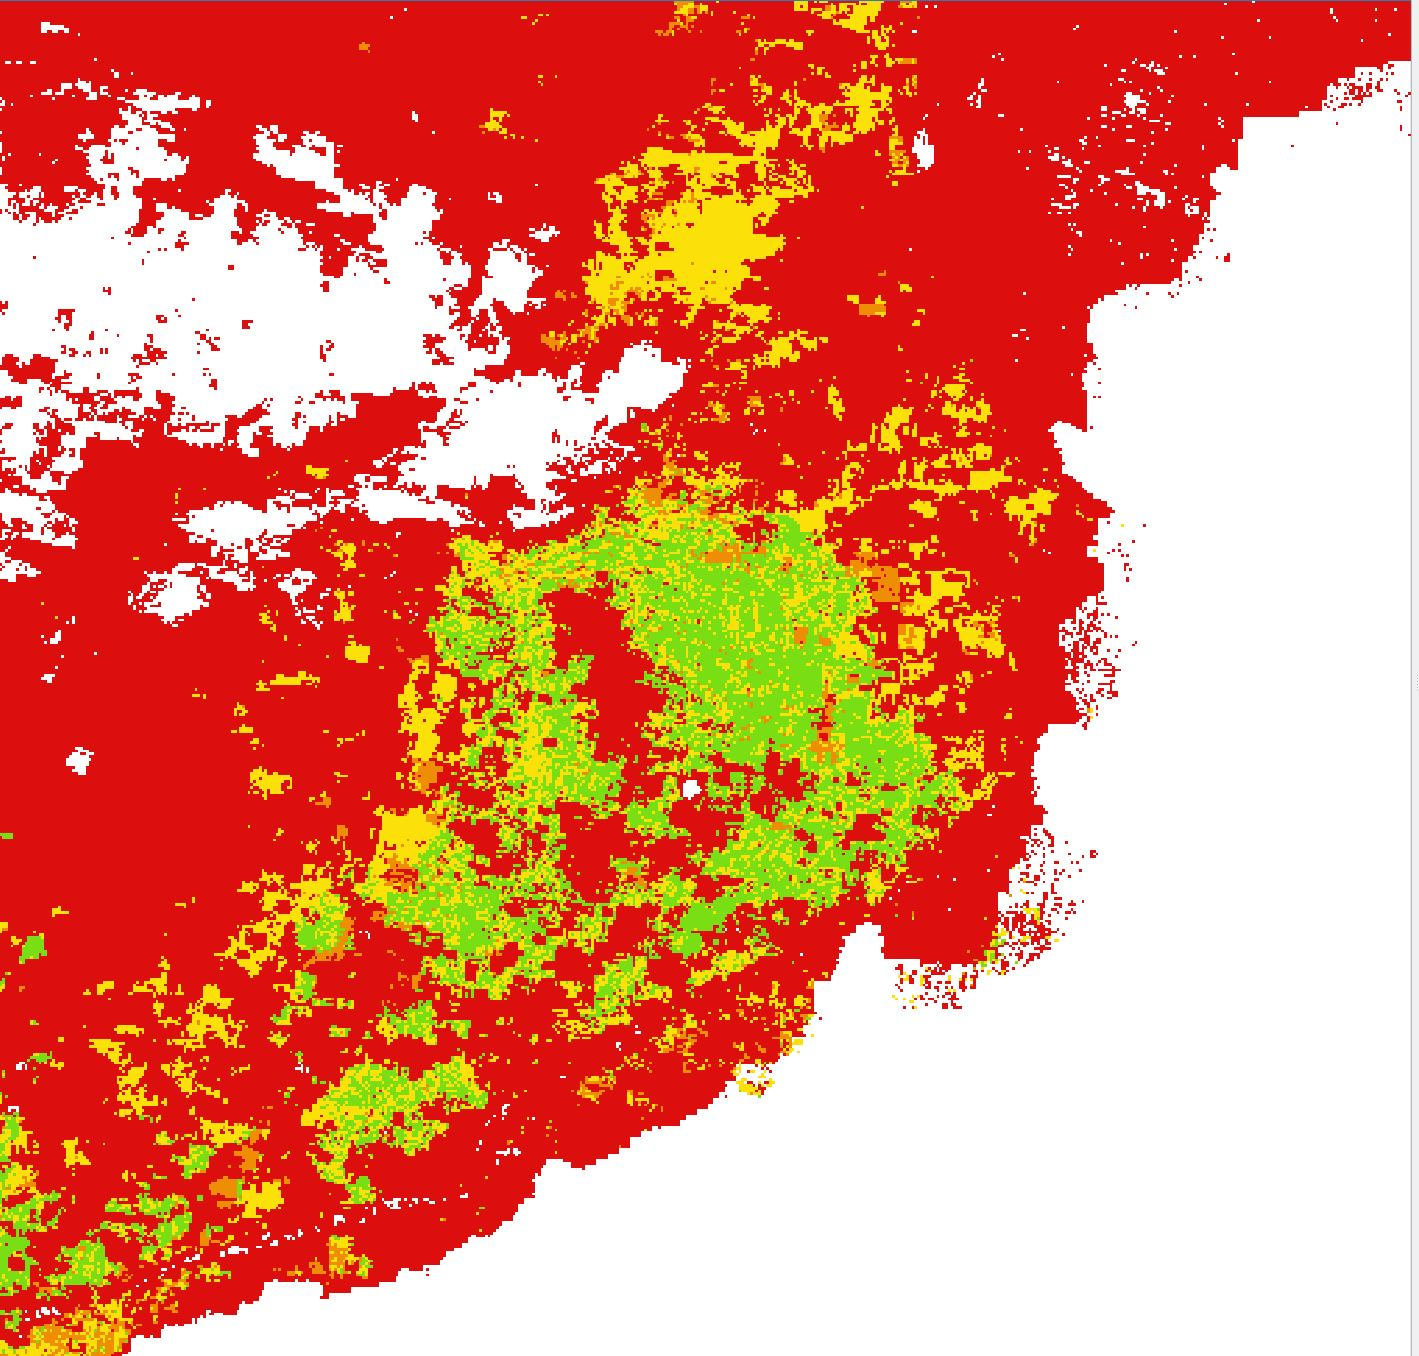
\includegraphics[scale=0.3]{./Grafiken/Fitting/Fitting_durchführung/Fitting_Vergleich_Rohdaten_Qualität_1.JPG}
\caption{\textit{Qualitätsinformtion für einen Auschnitt aus der Kachel h18v04 für den DOY 001 des Jahres 2001 - grün: full inversion - gelb: full inversion - orange: magnitude inversion ( numobs $>$=7)  - red: magnitude inversion ( numobs $2>$=7) - white: NoData}}
   \end{minipage}
\end{figure}

\begin{figure}[H] \label{fig:MODIS_data_jan}
\centering
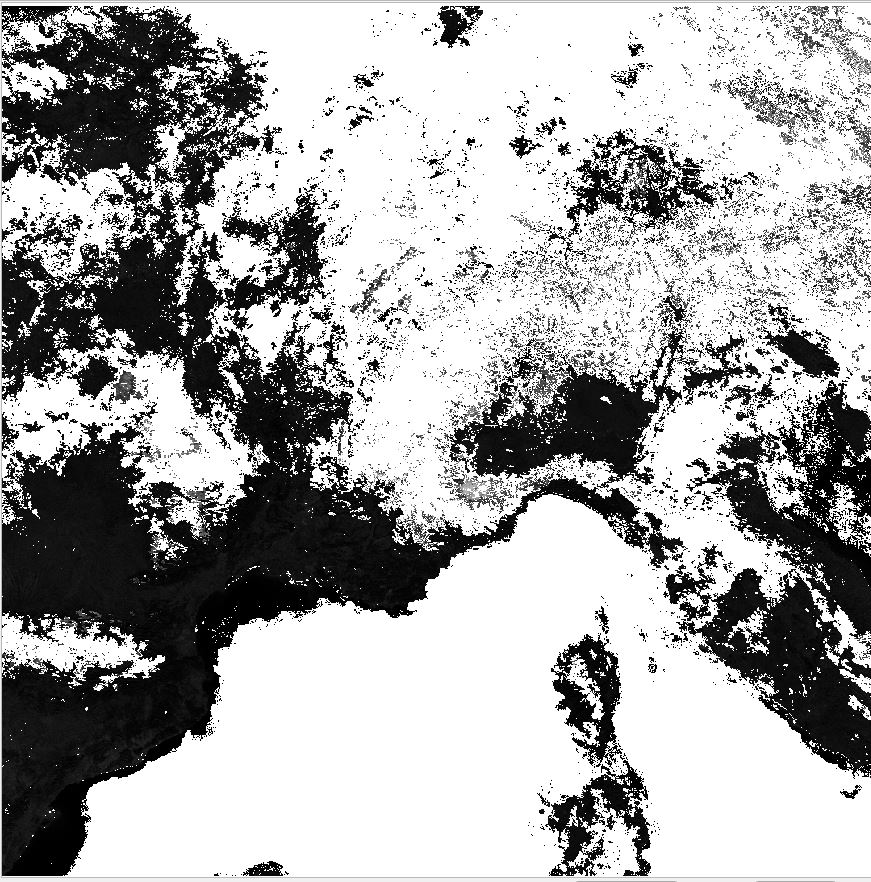
\includegraphics[scale=0.4]{./Grafiken/Fitting/Fitting_durchführung/Fitting_Vergleich_Rohdaten_Qualität_full_2.JPG}
\caption{\textit{Bildinformation für die Kachel h18v04 für den DOY 001 des Jahres 2001 - Weiss : NoData - Graustufen: Reflexionswerte}}
\end{figure}
\begin{figure}[H] \label{fig:MODIS_qual_jan}
\centering
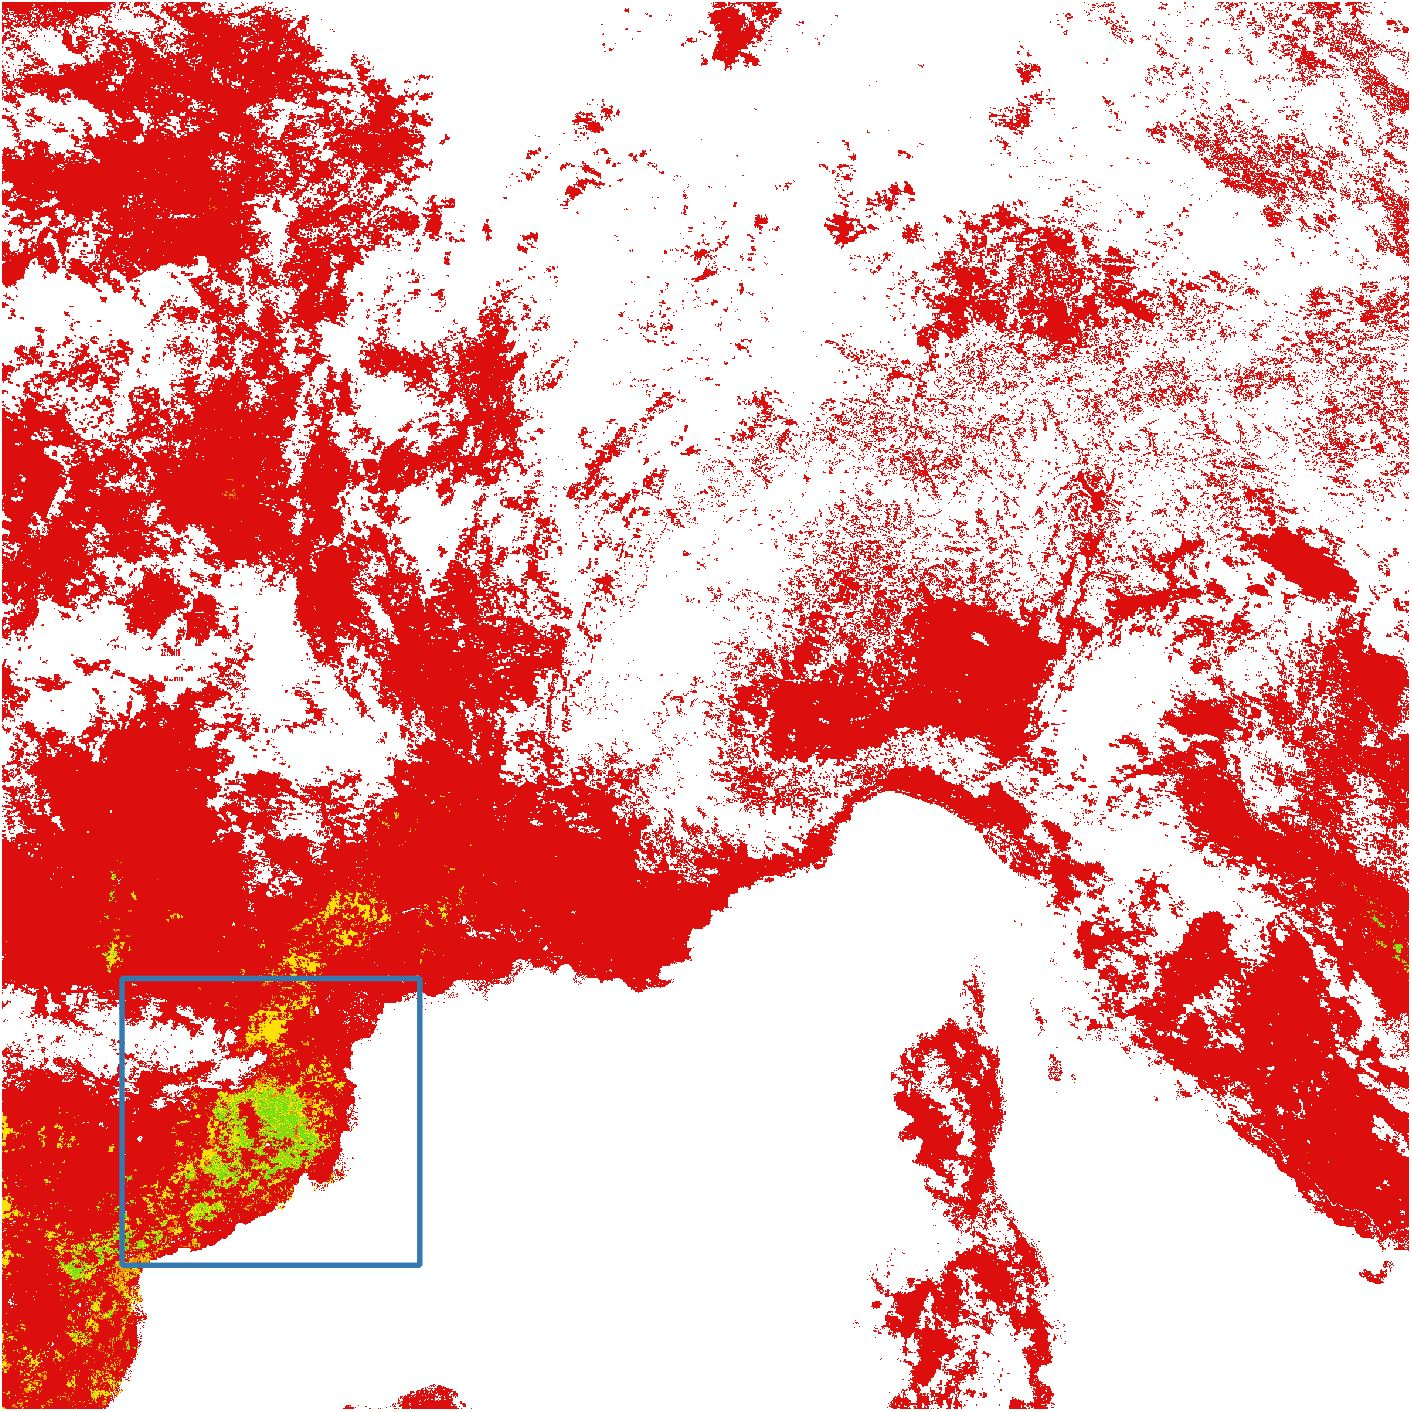
\includegraphics[scale=0.4]{./Grafiken/Fitting/Fitting_durchführung/Fitting_Vergleich_Rohdaten_Qualität_full_1.JPG}
\caption{\textit{Qualitätsinformtion für die Kachel h18v04 für den DOY 001 des Jahres 2001}}
\end{figure}

\subsection{Savitzky-Golay Filterung mit einem Polynom 2. Grades}
Wie schon in den Grundlagen angesprochen, verwendet eine Rekonstruktionsmethode den Savitzky-Golay-Filter um einerseits verrauschte Daten zu glätten als auch nicht vorhandene Daten zu rekonstruieren. Man wählt ein passendes sich bewegendes Zeitfenster aus, in diesem Fall werden 15 Beobachtungsepochen im Abstand von jeweils 8 Tagen verwendet, und updated dieses mit der nächsten Epoche nach abgeschlossener Filterung. Der zentrale Wert ( nicht der Median) innerhalb dieses Datenarrays ist der gefilterte Wert, welcher von Interesse ist und zur weiteren Bearbeitung und Verspeicherung herangezogen wird. Bevor es jedoch ans glätten der Zeitreihe geht wird überprüft, ob es NaN stellen im SG-Fenster gibt. Füllwerte treten abhängig vom Fortschritt des Jahres vermehrt in den niederschlagsreichen Zeiten, besonders gegen Ende und Anfang des Jahres auf. Auch der Rest des Jahres ist nicht davor gefeit keine NaN Werte zwischenzeitlich aufzuweisen. An diesen Stellen wird zu aller erst linear interpoliert, um einen Näherungswert für die anschließende Filterung an nicht besetzten Stellen zu haben. 
% Hier kommen die Plots von der Linearen interpolation für NaN Stellen - weiter im Code 
\begin{figure}[H]
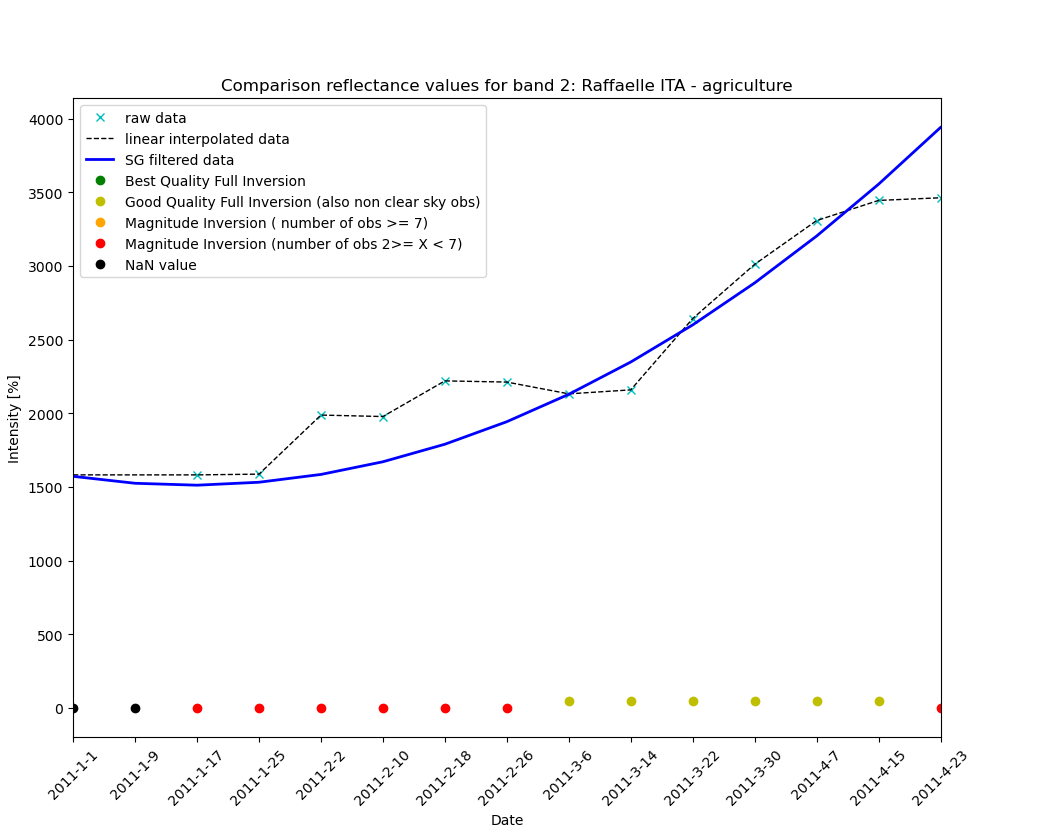
\includegraphics[scale=0.6]{./Grafiken/Fitting/Fitting_method_comparison/comparison_reflectance_values_for_band_2_raffaella_it.png}
\caption{\textit{Gegenüberstellung Rohdaten, lineare Interpolation, SG Filterung für einen Zeitraum von 15 Epochen im Raum Raffaelle Italien im NIR}}
\label{fig:compare_fit_sg_raf_it_2011}
\end{figure}
Abbildung \ref{fig:compare_fit_sg_raf_it_2011} stellt diese unterschiedlichen Zustände des Datenmaterials grafisch dar. Die unbearbeiteten Rohdaten sind als cyanfarbige X-Signaturen gekennzeichnet und deren Qualitätsklasse ist als farbige Punktsignatur am Fusse des Plotes dargestellt. Beste Qualität wird mit grün symbolisiert ( in \ref{fig:compare_fit_sg_raf_it_2011} ist keine vorhanden), gelb symbolisiert gute Qualität, sprich volle Inversion aber auch bewölkte Szenen werden mitverwendet,  orange beschreibt, dass mindestens 7 Beobachtungen für die Wertermittlung vorgelegen sind, rot das mindestens zwei Beobachtungen aber maximal 7 Beobachtungen zur Wertermittlung herangezogen wurden. Schwarz sind NoData Werte welche nicht zur Berechnung herangezogen werden können. Diese NoData Stellen werden mittels einer linearen Interpolation aus dem vorangegangenem und nachfolgendem Wert approximiert, um einen Näherungswert für die Filterung nach SG zur Verfügung zu haben. In Abbildung \ref{fig:compare_fit_sg_raf_it_2011} wird diese Approximation mittels der schwarzen gestrichelten Linie dargestellt. Dies ist nun die vollbesetzte Zeitreihe die zur Schätzung der Parameter des Polynom zweiten Grades wie in Formel \ref{form_poly_2nd}, welches für den Savitzky-Golay-Filter verwendet, herangezogen wird. Die durchgezeichnete blaue Linie symbolisiert die gefilterte Zeitreihe unter Verwendung des SG Filters mit einem 15 tägigem Beobachtungsfenster. Die Beobachtungen wurden nach absteigender Qualität mit 
\begin{itemize}
\item Best Quality = 1 
\item Good Quality = 0.5
\item Magnitude Inversion ( number of obs >= 7) = 0.25
\item Magnitude Inversion (number of obs 2>= X < 7) = 0.01
\end{itemize}


\subsection{DFT}
\subsection{FFT}
\end{document}
